% Fix: From https://tex.stackexchange.com/a/508995/108670
\RequirePackage{snapshot}
\makeatletter
\def\snap@providesfile#1[#2]{%
  \wlog{File: #1 #2}%
  \if\expandafter\snap@graphic@test\expanded{#2}@@\@nil
    \snap@record@graphic#1\relax #2 (type ??)\@nil
  \else
    \expandafter\xdef\csname ver@#1\endcsname{#2}%
  \fi
  \endgroup
}
\makeatother

\documentclass[twoside,a4paper,11pt]{memoir}
\usepackage{document}
\usepackage{minted}
\usepackage{subcaption}
\usepackage{listings}
\usepackage{xcolor}

\newcounter{oldtocdepth}
\newcommand{\hidefromtoc}{%
  \setcounter{oldtocdepth}{\value{tocdepth}}%
  \addtocontents{toc}{\protect\setcounter{tocdepth}{-10}}%
}
\newcommand{\unhidefromtoc}{%
  \addtocontents{toc}{\protect\setcounter{tocdepth}{\value{oldtocdepth}}}%
}

\definecolor{codegreen}{rgb}{0,0.6,0}
\definecolor{codegray}{rgb}{0.5,0.5,0.5}
\definecolor{codepurple}{rgb}{0.58,0,0.82}
\definecolor{backcolour}{rgb}{0.95,0.95,0.92}
\definecolor{num_color}{HTML}{0A6E2B}
\definecolor{kw_alt}{HTML}{1817A2}

\lstdefinestyle{mystyle}{
    backgroundcolor=\color{backcolour},   
    commentstyle=\color{codegreen},
    keywordstyle=\color{magenta},
    numberstyle=\tiny\color{codegray},
    stringstyle=\color{codepurple},
    basicstyle=\ttfamily\footnotesize,
    breakatwhitespace=false,         
    breaklines=true,                 
    captionpos=b,                    
    keepspaces=true,                 
    numbers=left,                    
    numbersep=5pt,                  
    showspaces=false,                
    showstringspaces=false,
    showtabs=false,                  
    tabsize=2
}

\lstset{style=mystyle}

% Add \@ _before_ the terminating period of the sentence (`UI\@. Test`)
% to allow inter-sentence spacing when the sentence ends with a capital letter.

\addbibresource{document.bib}
\addbibresource{researchr.bib}

% !TEX root = document.tex

\title{Generic Traversal Fusion in Strategic Programming}
\subtitle{Version of \today}
%\subtitle{Master's Thesis}
\author{Gijs van der Heide}
\authoremail{\url{vanderheidegijs1@gmail.com}}
\birthplace{Amersfoort, the Netherlands}
\studentid{5581672}
\coverpicture{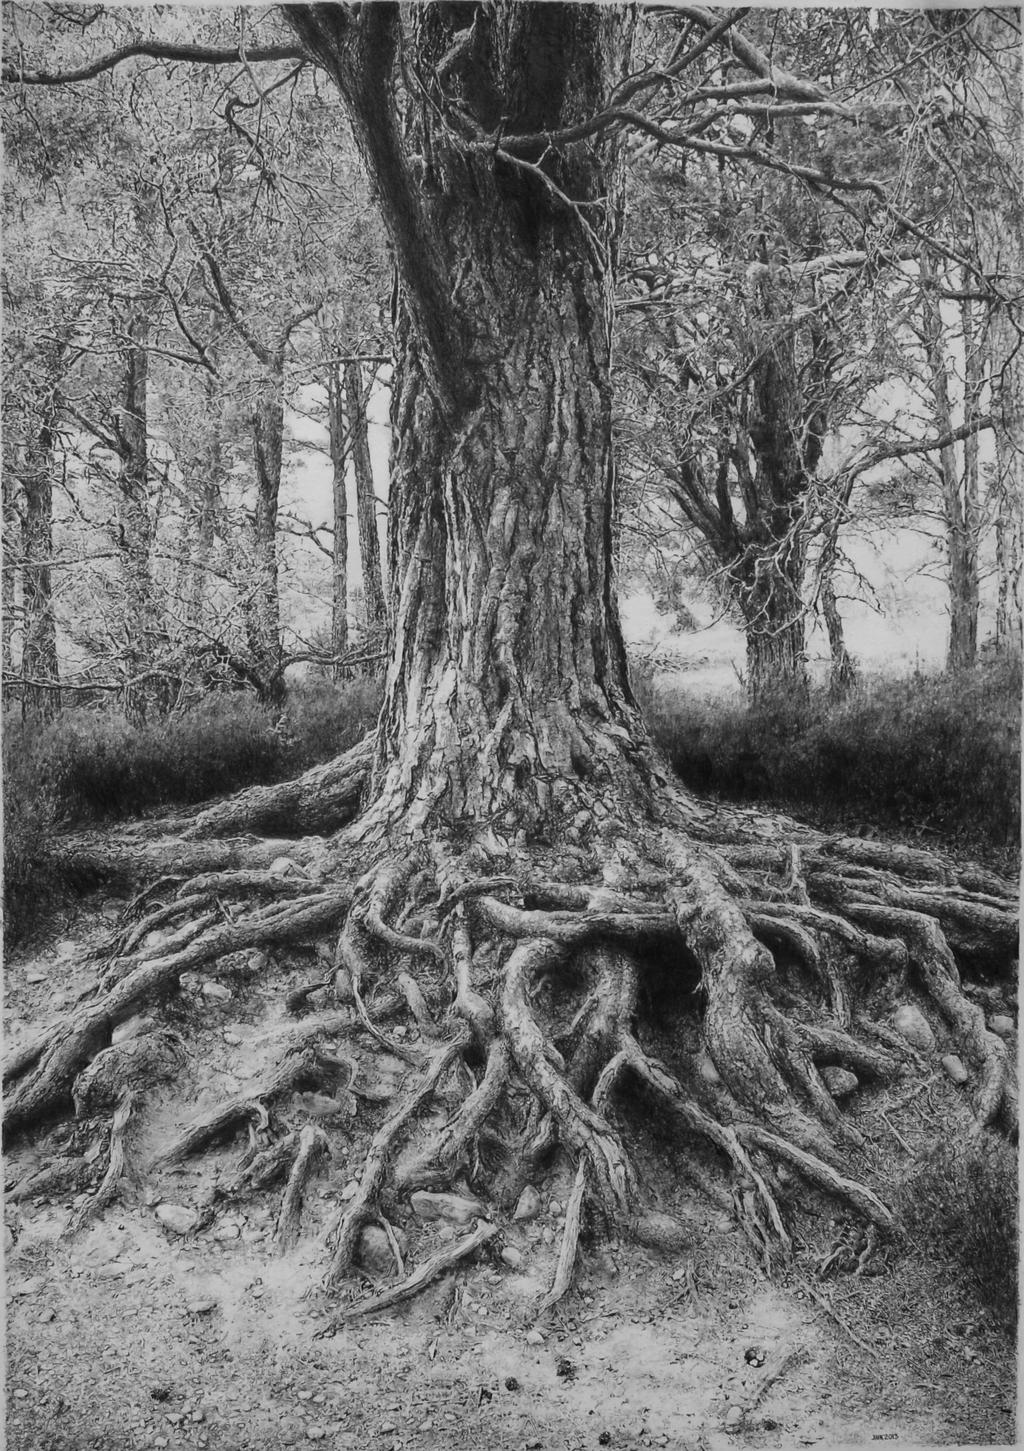
\includegraphics[width=10cm]{./img/tree_drawing.jpg}}
\colophon{\noindent
  \copyright{} \the\year{} \: \theauthor. \\[1em]
  An AI model by Writefull has been used in several places throughout this thesis for the sole purpose of grammar checking and suggestions. No AI has been used in the creation of any of the actual content of this thesis.\\[1em]
  Cover picture: \textit{"Tree drawing"}. By absolutemadman on DeviantArt. Licensed under CC BY-NC-ND. https://www.deviantart.com/absolutemadman/art/Tree-drawing-365459720
}


\begin{document}

\frontmatter
\thispagestyle{empty}
\maketitle
\makeformaltitlepages{% !TEX root = document.tex

Traversing and transforming tree-like data structures is a common occurrence in developing compilers, interpreters, and other program transformation or analysis tools. In more complex programs, multiple traversals are often performed on the same tree, leading to potentially unnecessary repeated visits of nodes. Finding opportunities to reduce repeated visits is an optimization called traversal fusion.

Tree traversals are particularly common in the strategic programming paradigm. In this paradigm, the transformations that are performed are separated from the manner in which trees are traversed, enabling simple and scalable control over traversals \cite{LaemmelVV02}. We consider traversal fusion as an optimization for strategic programming languages.

We developed an algorithm to perform traversal fusion in strategic programming languages. Our algorithm is based on TreeFuser and Grafter \cite{SakkaS017, SakkaSN019}, two related algorithms developed in previous work on imperative programs. The algorithm performs dependency analysis on strategic programs, and then attempts to fuse together recursive calls without introducing dependency violations in order to determine legal opportunities for traversal fusion.

We developed a proof-of-concept (POC) implementation of this algorithm to work on a subset of the Stratego programming language. We evaluated this POC on a synthetic benchmark that mimics real-world usages of strategic programming, as well as a best-case scenario benchmark, to assess the viability and benefit of this optimization for strategic programming languages.

In the best-case scenario benchmark, we measure a mean runtime decrease of 48\%. In a benchmark simulating rendering a web page by traversing a render tree, the total number of tree node visits is reduced by over 40\%. While we measure a similar performance benefit for this benchmark initially, we find that this is caused by code synthesis, unrelated to fusion. There is no measurable additional performance increase when enabling fusion. We determine that this is most likely caused by overhead when fusing more complex programs, or relatively expensive other parts of the program dominating total runtime.

In conclusion, we find that traversal fusion is possible in strategic programming, but several factors can reduce real-world performance impact, limiting its viability as an optimization. We make suggestions to further explore this optimization in the context of strategic programming.
}

% !TEX root = document.tex

\chapter{\label{chap:Preface}Preface}
\addcontentsline{toc}{subsection}{Preface}
When I sat behind my laptop writing Minecraft \textit{mods}\footnote{\textit{modifications}, that change or add to the popular sandbox video game, https://www.minecraft.net/} while watching Java tutorials on YouTube ten years ago, I never would have thought I would end up here, pursuing a degree in Computer Science. I enjoyed most, if not all, subjects taught in school, and on the one hand, I might say I could have ended up pursuing almost any other degree. Deciding what I wanted to do after high school was certainly not easy. On the other hand, looking back, the choice for Computer Science was perhaps inevitable. I remember how programming always had something unique: I enjoyed the problem solving aspect, but also the general idea of making such a mysterious machine do what \textit{I} wanted it to do.

Of course, I quickly realized that the field of Computer Science went a lot deeper than just programming when I arrived in Delft. But, in Delft too, I truly enjoyed almost every course. And at the same time, here too, some courses jumped out: courses focused on low-level programming and computer engineering (e.g. Computer Organization), as well as the more high-level, abstract courses such as Algorithm Design, or Concepts of Programming Languages.

When I finished my bachelor's, I had some doubts about whether I also wanted to pursue a master's. The additional years of education, life experience, and some changes in the field, as well as the world in general, meant I suddenly saw a lot of different options. At the same time, I had really enjoyed the last three years. And because I reject that the sunk cost fallacy is a fallacy, I managed to convince myself that one is not really supposed to do a bachelor's without then doing the master's.

And so, I enrolled. When I did, I decided almost immediately that I would be doing a thesis on a topic related to programming languages, because I had grown to enjoy those courses the most. Jeff's listing for this project was the second one I clicked, and it spoke to me immediately.

I think, looking back objectively, my motivation during the master's was definitely worse than it was during the bachelor's, but I certainly cannot blame this project for that. It was very interesting, as were my weekly meetings with Jeff. We rarely finished on time, but I usually had little else to do for the rest of the day. Jeff, of course, did... sorry! And, of course, thanks for all the help! I would also like to thank Jesper for his feedback, and Neil for joining the committee. Also, I would like to thank them all for being willing to work with me throughout the summer.

Of course, I must also thank my parents and stepparents, for all their support throughout the years. They made it possible for me to focus on my studies without having to worry too much about matters such as money, having a place to live, etc. These things feel normal to me, but I know, of course, that they aren't normal for everyone. As such, I am very grateful for them.

And so, we arrive at the end of the master's. Perhaps fittingly, I once again am faced with doubts about what I want to do now. I have decided that I will not be pursuing a career in academics or really even the field of Computer Science in general. It does feel a little strange, closing this chapter of my life, and `never looking back', in a sense. Of course, I know I will look back: I think my education at the TU has been and will always be incredibly valuable, and I can truthfully say I do not regret any of my choices. Besides the effects of just getting older, I think my five years at the TU have changed me as a person, and perhaps in that sense have caused me to now pursue something different. Well, such is life.

\vspace{1cm}
\begin{flushright}
\theauthor{}\\
Baarn, the Netherlands\\
August 19, 2026\\
\end{flushright}


\cleardoublepage\tableofcontents
\cleardoublepage\mainmatter{}

% !TEX root = document.tex

\lstdefinestyle{mystyle_bt_basic}{
language = Python,
otherkeywords = {E, Null, 0, 1, 2, 3, 4, 5, 6},
keywordstyle = [2]{\color{num_color}},
morekeywords = [2]{0, 1, 2, 3, 4, 5, 6}
}
\lstdefinestyle{mystyle_bt_basic_stratego}{
language = Python,
otherkeywords = {r-zero, 0},
morekeywords = {E, Exp, Null, program},
keywordstyle = [2]{\color{num_color}},
morekeywords = [2]{0},
keywordstyle = [3]{\color{kw_alt}},
morekeywords = [3]{constructors, rules, strategies, topdown, Int}
}
\lstdefinestyle{mystyle_increment_comparison}{
language = Python,
otherkeywords = {r-increment5, r-increment1},
morekeywords = {E, S, program},
keywordstyle = [2]{\color{kw_alt}},
morekeywords = [2]{rules, strategies, topdown}
}
\lstdefinestyle{mystyle_copy_up}{
language = Python,
otherkeywords = {r-copy-up},
morekeywords = {E, Null}
}

\chapter{Introduction}
\label{chap:introduction}
Traversing and transforming tree-like data structures is a common occurrence in developing program analysis tools, refactoring tools, and compilers or interpreters that operate on abstract syntax trees (AST's). Control over the application order of the transformations, the propagation of effects, and the traversal of the input data is often necessary to correctly implement more complex program transformations\autocite{LaemmelVV02}. Most programming paradigms provide limited support for separating traversal control from the rest of the program, limiting reusability and scalability\autocite{LaemmelVV02}.

Strategic programming languages address this challenge by separating the transformations that are performed from the manner in which trees are traversed. Users define rewrite rules that operate on trees, and strategies that determine how trees are traversed and when rewrite rules are applied. These strategies are also generic in the sense that they are polymorphic: a single definition of the strategy is enough to work on any type of node \autocite{LaemmelVV02, Visser01}.

In more complex programs operating on tree-like data structures, multiple traversals are often performed on the same tree, leading to potentially unnecessary repeated visits of nodes. Identifying traversals that can be fused together safely reduces repeated visits and thus runtime overhead. This optimization is called traversal fusion.

Strategic programming languages, while intuitive and convenient to use in their domains, are high-level languages. The trade-off between convenient abstractions in high-level languages and computational performance in low-level languages is well-established \cite{SiskindP16a, Kovacs24}. At the same time, optimizing compilers can, in some cases, recover performance in high-level languages \cite{Mainland17}, and in many cases programs written in higher-level languages ``rely heavily on [these] optimizations to achieve adequate performance" \cite{Kovacs24}. In recent times, as Moore's law is seemingly coming to an end while Artificial Intelligence (AI) creates increasingly large performance demands, compiler optimizations may be more relevant than ever \cite{ZHANG2023}. Only  a small number of compiler optimizations are available for strategic languages, and these languages suffer from a general lack of research on how to improve their performance compared to more popular paradigms. We contribute to this problem by attempting to apply the traversal fusion optimization in strategic programming.

The number of fusion opportunities, as well as the amount of runtime overhead due to repeated visits, depend on the program being analyzed and can vary significantly between different programs. A program could theoretically have no fusion opportunities at all, or arbitrarily many. The best-case scenario for the traversal fusion optimization is a program with a large number of traversals that perform different, non-conflicting operations. The possible performance increase due to traversal fusion further depends on the input size. The traversal fusion optimization is ideal for tree traversal programs that are compiled once and then run on many different inputs, such as program transformation tools. In such a scenario, the increased compile time is a one-time investment that can, in a sense, be amortized over all subsequent executions of the program. Previous work on imperative programs has shown that traversal optimization is effective for real-world program transformation use cases: Grafter can achieve speedups between 1.5 and 4.5 times in a render tree transformation benchmark, with larger input sizes achieving a greater speedup \cite{SakkaS017, SakkaSN019}. 

However, this is no guarantee that the optimization is effective for strategic programming. Even if the same analysis can be performed, and the same fused traversal implemented, strategic languages have different data representations, different ways of implementing traversals, and different sources of overhead. If it is effective in strategic programming, we hope that it could be one of many optimizations that gradually increase the performance of strategic programming languages and consequently increase the adaptation of the paradigm.

\section{Stratego}
In this thesis, we focus mainly on the strategic programming language Stratego, originally developed around 2001 \autocite{Visser01}, and currently still in development at the Delft University of Technology. Stratego allows users to specify rewrite rules, strategies, and input data in Annotated Terms (ATerms). ATerms are a simple and efficient way to represent tree-like data structures \autocite{BrandJKO00}.

As an example, consider the binary tree of integers and its ATerm representation shown in \autoref{fig:binary-tree-basic}, as well as \autoref{fig:binary-tree-basic-stratego}, which shows how to define such a tree in Stratego, and how to perform a basic operation on it.

\begin{figure}
\centering

\begin{subfigure}{0.5\textwidth}
    \centering
    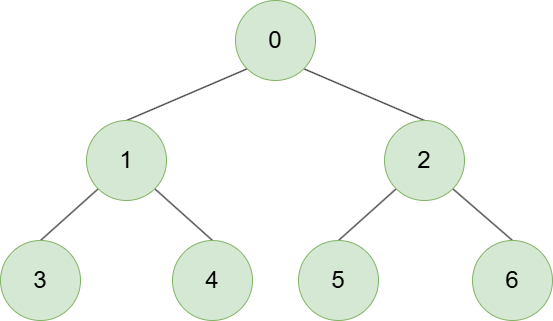
\includegraphics[width=6cm]{./img/binary-tree-basic.png}
    \subcaption{Binary tree of integers}
\end{subfigure}%
\begin{subfigure}{0.5\textwidth}
\centering
\begin{lstlisting}[style=mystyle_bt_basic]
    E(0,
      E(1,
        E(3, Null(), Null()), E(4, Null(), Null())
      ),
      E(2,
        E(5, Null(), Null()), E(6, Null(), Null()
      )
    )
\end{lstlisting}
    \subcaption{ATerm representation}
\end{subfigure}

\caption{A binary tree of integers and its ATerm representation.}
\label{fig:binary-tree-basic}
\end{figure}

To define a binary tree the constructors \texttt{E} and \texttt{Null} are defined. The constructor \texttt{E} represents nodes that contain an integer, and that have two children that are also \texttt{E} nodes, or \texttt{Null} if the node is a leaf.

\begin{figure}
\begin{lstlisting}[style = mystyle_bt_basic_stratego]
    constructors
      E: Int * Exp * Exp -> Exp
      Null: Exp

    rules
      r-zero:
        E(v, l, r) -> E(0, l, r)

    strategies
      program = topdown(r-zero)
\end{lstlisting}
\caption{A binary tree and an operation on it, defined in Stratego.}
\label{fig:binary-tree-basic-stratego}
\end{figure}

As an example of an operation that can be performed on this tree, a rewrite rule is defined in \autoref{fig:binary-tree-basic-stratego} that sets the value of every node to zero. This rule sets the first child (the \texttt{v} field) to 0, but does not recursively apply itself to the children \texttt{l} and \texttt{r}. Instead, this traversal logic is factored out of the rule into a generic traversal. To apply this rule to the entire tree, all we have to do is call the \texttt{topdown} strategy. The \texttt{topdown} strategy takes a rule, applies it to the current node, and then applies it to each of that node's children recursively and generically. 

\texttt{topdown} is just one of many available strategies in Stratego, and users can also define their own strategies. This small example already shows one of the main benefits of strategic programming: adding a new type of constructor to this tree would not require any changes to the traversal logic, unless different behavior was specifically desired for that constructor.

\section{Traversal Fusion}
In Stratego, users can easily write programs consisting of sequences and combinations of traversals that can perform complex operations on trees. This is quite useful: for example, a user might simply want to apply a set of rules to a tree, and then another set, and then another. This can be expressed naturally in just a few lines of code. Or, consider a program transformation that performs a simplification: applying such a rule once may introduce new opportunities for simplification. Thus, such a rule might have to be applied repeatedly until the tree no longer changes.

However, the ease with which more traversals can be added into a Stratego program does raise the question of whether this is always efficient. Consider applying a single rule top-down multiple times in a row on the same tree. It is very easy to simply call \texttt{topdown} multiple times. But in some cases it might also be possible to change the rewrite rule itself to still do everything in a single traversal. As the input data get larger, the traversals themselves start taking up a considerable amount of the program runtime through memory accesses. Performing fewer traversals would reduce the number of times nodes are visited, and thus also the number of memory accesses. For very large input data, reducing the number of unique node visits also reduces cache misses, which have a significant performance impact. In theory, then, performing fewer traversals should be faster.

This means that users, especially when writing more complex programs, do have to think about how their rewrite rules and traversals interact. This seems somewhat counter to the objective of strategic programming languages to separate these things. In many cases, the version of a program with fewer traversals might also be more complex or less intuitive to write. As such, automatically identifying opportunities for traversal fusion is an interesting and promising optimization for strategic programming. It is important to note that traversal fusion does \textit{not} change the rewrite rules, and achieves fusion in a different way. The time savings come from the reduction in overhead created by the memory accesses of the traversals. Fewer traversals after fusion lead to less overhead.

\subsection{Example of Legal and Illegal Fusion}
Consider the example shown in \autoref{fig:increment-by-five-comparison}. In this example, we want to apply a rule that increments the values in a binary tree of integers by five. This can be done efficiently in a single top-down traversal applying a single rewrite rule that increments the values by five (\autoref{fig:increment-by-five-comparison-1}). It can also be done by performing five top-down traversals in a row, each applying a rewrite rule that increments values by one (\autoref{fig:increment-by-five-comparison-2}). The traversal fusion optimization would analyze the latter program and determine that these five traversals can safely be fully fused together. In this case, a program that only goes through the tree top-down once, applying the rewrite rule five times in a row at every node, has equivalent behavior (\autoref{fig:increment-by-five-comparison-3}).

\begin{figure}

\begin{subfigure}{\textwidth}
\begin{lstlisting}[style = mystyle_increment_comparison]
    rules
      r-increment5 :
        E(v, l, r) -> E(S(S(S(S(S(v))))), l, r)
    
    strategies
      program = topdown(r-increment5)
\end{lstlisting}
\subcaption{Single traversal, with a single rewrite rule}
\label{fig:increment-by-five-comparison-1}
\end{subfigure}

\begin{subfigure}{\textwidth}
\begin{lstlisting}[style = mystyle_increment_comparison]
    rules
      r-increment1 :
        E(v, l, r) -> E(S(v), l, r)
    
    strategies
      program = topdown(r-increment1); topdown(r-increment1);
        topdown(r-increment1); topdown(r-increment1); topdown(r-increment1)
\end{lstlisting}
\subcaption{Five traversals}
\label{fig:increment-by-five-comparison-2}
\end{subfigure}

\begin{subfigure}{\textwidth}
\begin{lstlisting}[style = mystyle_increment_comparison]
    rules
      r-increment1 :
        E(v, l, r) -> E(S(v), l, r)
    
    strategies
      program = topdown(r-increment1; r-increment1;
        r-increment1; r-increment1; r-increment1)
\end{lstlisting}
\subcaption{Single traversal, fused from five traversal version}
\label{fig:increment-by-five-comparison-3}
\end{subfigure}

\caption{Comparison of increment-by-five programs.}
\label{fig:increment-by-five-comparison}
\end{figure}

Finding fusion opportunities is not always this simple. As seen in the previous example, consecutive traversals writing to the same field does not necessarily prevent fusion. Problems generally arise when traversals use information stored in nodes \textit{other} than the current node. The intuitive reasoning behind this is that traversal fusion alters a program's execution order, and other nodes may be in invalid states. For example, when executing the fused increment program, the current node may have a value of $5$, while its children all sit at $0$. In the unfused program that performs five traversals, values never differ by more than $1$.

As a concrete example of when fusion is not legal, define a rewrite rule that copies the value of a node's child into that node, as shown in \autoref{fig:twotd-counterexample-1}.

\begin{figure}

\begin{subfigure}{\textwidth}
\begin{lstlisting}[style = mystyle_copy_up]
    r-copy-up:
      E(_, E(v, c)) -> E(v, E(v, c))

    r-copy-up:
      E(v, Null()) -> E(v, Null())
\end{lstlisting}
\subcaption{\texttt{copy-up} rewrite rule}
\label{fig:twotd-counterexample-1}
\end{subfigure}

\begin{subfigure}{0.5\textwidth}
\centering
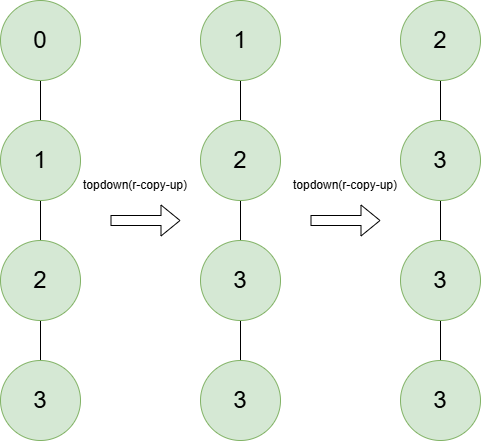
\includegraphics[width=6.5cm]{./img/twotd-counterexample-unfused.png}
\subcaption{Two top-down traversals in a row}
\label{fig:twotd-counterexample-2}
\end{subfigure}%
\begin{subfigure}{0.5\textwidth}
\centering
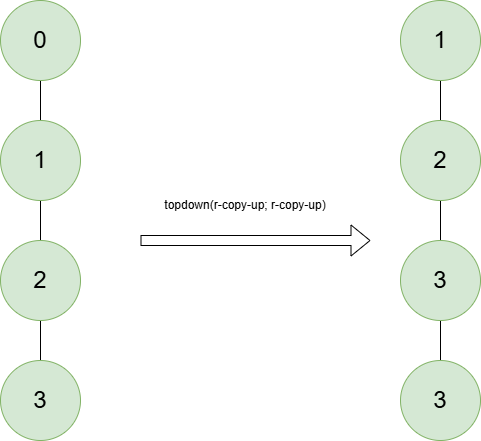
\includegraphics[width=6.5cm]{./img/twotd-counterexample-fused.png}
\subcaption{Single top-down traversal}
\label{fig:twotd-counterexample-3}
\end{subfigure}

\caption{Counter-example to the fusion of two top-down traversals.}
\label{fig:twotd-counterexample}
\end{figure}

Executing this rule twice top-down on an example tree gives the result shown in \autoref{fig:twotd-counterexample-2}. However, fusing the top-down traversals into a single top-down traversal results in \autoref{fig:twotd-counterexample-3}, which is not the same. The intuition here is that the second application of the rewrite rule in the fused version does not actually do anything. It simply copies up the value of the child again, but that value cannot have changed. In the unfused version, that value \textit{has} changed (except in the case of the leaf), because the rewrite rule has already been applied once to that child.

\section{This Thesis}
Using information stored in other nodes does not always prevent fusion. Determining when it (or another effect) does and does not prevent fusion is exactly the problem of automated traversal fusion. Traversal fusion is not a totally new concept, and some research has been done on this topic. For example, research has been done on very specific fusions in Stratego that are always possible \autocite{JohannV01}. More general traversal fusion has also been achieved in other contexts, for example with circular programming \autocite{FernandesPS07}, or using dependency analysis \autocite{SakkaS017, SakkaSN019}. We will focus on the dependency analysis approach in this thesis. Other related work is discussed in more detail in \autoref{chap:rw}.

None of the research that has been done, however, applies directly to strategic programming and fusing generic traversals. It is not clear whether this can be done at all in strategic programming, how it might be done, and what its potential benefit might be.

The research question for this thesis is: `Can generic traversal fusion be performed in strategic programming languages, and what is the impact of this optimization on strategic programs?'

We make the following contributions in this thesis:
\begin{itemize}
    \item We develop an algorithm that can apply the traversal fusion optimization in strategic programming languages based on the TreeFuser and Grafter algorithms\cite{SakkaS017, SakkaSN019}. It can analyze the dependencies of a set of traversals and rewrite rules, and synthesize a fused traversal if one exists.
    \item We implement a proof-of-concept (POC) traversal fusion optimizer using this algorithm that works on a subset of the Stratego language. This POC supports simple constructors (e.g. no list types), rewrite rules without side effects (function calls are allowed), and a single sequence of operations consisting of any combination of calls to \texttt{all}, rule applications, calls to \texttt{topdown} or \texttt{bottomup}, or calls to other strategies using only these features.
    \item We evaluate the POC on a synthetic benchmark simulating the rendering of a web page to determine the real benefit of this optimization in strategic programming. We find that it effectively reduces node visits by over 40\%, while not having measurable impact on runtime or memory usage. While a runtime improvement is technically present, it is caused by our code synthesis and not the fusion. Under some circumstances (e.g. when performing full fusion), traversal fusion can have a measurable performance impact in strategic programming, but these situations are less likely to occur in real-world usage.
\end{itemize}
% !TEX root = document.tex

\lstdefinestyle{mystyle_regex_comparison}{
language = Python,
otherkeywords = {simpl-rule},
morekeywords = {Choice, Epsilon, Option, Plus, Star, simpl},
keywordstyle = [2]{\color{kw_alt}},
morekeywords = [2]{topdown}
}
\lstdefinestyle{mystyle_small_stratego_listings}{
language = Python,
otherkeywords = {match_a, match_b, match_any_1, match_any_2, do_something_with_A, do_something_with_B, my_strategy, function_1, function_2},
morekeywords = {A, B, C},
keywordstyle = [2]{\color{kw_alt}},
morekeywords = [2]{topdown, all, try, id, fail}
}
\lstdefinestyle{mystyle_map_rule_haskell}{
language = Haskell
}
\lstdefinestyle{mystyle_map_rule_stratego}{
language = Python,
otherkeywords = {r-increment, r-mult, 1, 2},
morekeywords = {E, f},
keywordstyle = [2]{\color{num_color}},
morekeywords = [2]{1, 2},
keywordstyle = [3]{\color{kw_alt}},
morekeywords = [3]{topdown}
}
\lstdefinestyle{mystyle_grafter_example}{
language = Python,
keywordstyle = \color{kw_alt},
keywordstyle = [2]{\color{magenta}},
morekeywords = [2]{increment, multiply, fused_traversal}
}

\chapter{\label{chap:background}Background}
In this chapter, we give background information on the problem of (generic) traversal fusion, and introduce terminology that is useful in working towards a solution for fusion in strategic programming. In addition, we discuss TreeFuser and Grafter: the research on which our solution is based\autocite{SakkaS017, SakkaSN019}. Specifically, we will discuss:

\begin{itemize}
    \item What exactly is a traversal in strategic programming, and what do traversals look like in Stratego?
    \item What exactly does it mean to fuse traversals, and why is it not a trivial problem?
    \item How do TreeFuser and Grafter implement traversal fusion \autocite{SakkaS017, SakkaSN019}?
\end{itemize}

\section{Traversals}
First, we briefly contrast functional programming and strategic programming to show how the separation of rewrite rules and traversals makes strategic programming intuitive when operating on tree-like data structures.

In functional languages, users must explicitly program the order and location in which functions have to be executed to perform a rewrite on input data. This makes the evaluation strategy explicit, but does entangle it with the actual computations. In strategic programming, the evaluation strategy (i.e., traversals) and the computation (i.e., rewrite rules) are separated \autocite{LaemmelVV02}. As an example, consider the comparison of a simplification performed on regular expressions between Haskell and Stratego shown in \autoref{fig:regex-comparison} \autocite{LaemmelVV02}.

\begin{figure}

\begin{subfigure}{\textwidth}
\begin{lstlisting}[language=Haskell, otherkeywords={::, ->, =}, morekeywords={RegExp, Choice, Epsilon, Option, Plus, Star, Seq}]
    simpl :: RegExp -> RegExp
    
    -- rewrite rules
      -- eps | e - > e?
    simpl (Choice Epsilon e) = Option (simpl e)
      -- (e+)? - > e*
    simpl (Option (Plus e)) = Star (simpl e)
    
    -- traversal
    simpl (Star e) = Star (simpl e)
    simpl (Plus e) = Plus (simpl e)
    simpl (Option e) = Option (simpl e)
    simpl (Seq e1 e2) = Seq (simpl e1) (simpl e2)
    simpl (Choice e1 e2) = Choice (simpl e1) (simpl e2)
    simpl e = e
\end{lstlisting}
\subcaption{In Haskell}
\label{fig:regex-comparison-haskell}
\end{subfigure}

\begin{subfigure}{\textwidth}
\begin{lstlisting}[style = mystyle_regex_comparison]
    simpl-rule :
        Choice(Epsilon, e) -> Option(e)
        
    simpl-rule :
        Option(Plus(e)) -> Star(e)
        
    simpl = topdown(simpl-rule)
\end{lstlisting}
\subcaption{In Stratego}
\label{fig:regex-comparison-stratego}
\end{subfigure}

\caption{Comparison of a regular expression simplification program between Haskell and Stratego.}
\label{fig:regex-comparison}
\end{figure}

In the Haskell program, the traversal into every possible constructor has to be explicitly defined. Additionally, the \texttt{simpl} function has to be called in the rewrite rules to make sure the simplification continues to traverse down the AST. In contrast, the rewrite rules and traversal are completely separated in the Stratego program. On top of that, the traversal is also defined generically in the Stratego program: \texttt{topdown} works for all constructors.

\subsection{Definition}
We now define exactly what we mean by a traversal, or a strategy in Stratego. There is a subtle difference between the terms traversal and strategy: a traversal is a specific way to iterate over a data structure. A strategy is the way to define a traversal on a data structure in a strategic programming language. For the purposes of traversal fusion, talking about the traversal or the strategy that defines it usually does not cause confusion. For example, Stratego's \texttt{topdown} strategy defines a top-down traversal. The algorithm we have developed fuses traversals, but these traversals are \textit{represented} as strategies.

Strategies do have some specific properties that are important to mention. Strategies are \autocite{LaemmelVV02}: 

\begin{itemize}
    \item \textbf{Generic} - applicable to data of any shape;
    \item \textbf{Specific} - provide access to data structures on which they operate;
    \item \textbf{Partial} - may fail;
    \item \textbf{First-class} - they can be named and passed as arguments,
\end{itemize}

\noindent and enable

\begin{itemize}
    \item \textbf{Traversal} - generic traversal into subcomponents of data structures;
    \item \textbf{Control} - can model control over the application of computations (i.e. the application of rewrite rules).
\end{itemize}

These properties define the basic building blocks that can be used to define traversals in any strategic language.

\subsection{Stratego Traversals}
There are six basic strategy building blocks that arise from the aforementioned properties for any strategic programming language \autocite{LaemmelVV02}. These are also exactly the building blocks available in Stratego. Because these building blocks are the essence of the way to define traversals in Stratego, they will be used extensively in this thesis. We will list them here, and show how they might be used to define some basic strategies, or traversals. The six building blocks are:

\begin{itemize}
    \item Identity (\texttt{id}) - always succeeds and does nothing when applied to any term
    \item Failure (\texttt{fail}) - always fails when applied to any term
    \item Sequence (\texttt{\_;\_}) - first applies its left-hand argument, then applies its right-hand argument to a term
    \item Conditional (\texttt{\_<\_;\_}) - Attempts to apply its first argument. If this succeeds, it then applies its second argument to the result. Otherwise, it applies its third argument to the original term.
    \item All (\texttt{all(\_)}) - Applies its argument to all (direct) children of the current term. Fails if any application fails.
    \item One (\texttt{one(\_)}) - Attempts to apply its argument to all (direct) children of the current term, but stops upon the first successful application. Fails if all applications fail.
\end{itemize}

In addition to having these building blocks available, it is also legal to use recursive definitions in Stratego. This enables the definition of several important strategies, such as \texttt{topdown}:

\begin{lstlisting}[style = mystyle_small_stratego_listings]
    topdown(s) = s; all(topdown(s))
\end{lstlisting}

\noindent The \texttt{topdown} strategy takes one argument, \texttt{s}. When applying the \texttt{topdown} strategy to a node, it uses the sequence operator (\texttt{;}) to first apply \texttt{s} to that node. Then, it uses \texttt{all} to apply \textit{itself} to all children of the node. Indeed, this strategy exactly defines a top-down traversal.

Another useful strategy is \texttt{try}. This strategy attempts to apply its argument. However, if this fails, the \texttt{try} strategy itself does not fail:

\begin{lstlisting}[style = mystyle_small_stratego_listings]
    try(s) = s < id + id
\end{lstlisting}

\subsection{Additional Stratego Syntax}
\label{sec:additional-stratego-syntax}
We discuss two additional Stratego syntax features that are used in this thesis: matches and congruences.

First, matches allow for matching on a term inside a strategy. We use this to dynamically check the constructor of a node in our fused traversal functions, in combination with the conditional operator. The match operator is a question mark \texttt{?}. It succeeds if the match succeeds on the current node, and it fails if the match fails. For example, consider two constructors \texttt{A} and \texttt{B}, both with one subterm of type \texttt{Int}. The current node is \texttt{A(1)}. Then,

\begin{lstlisting}[style = mystyle_small_stratego_listings]
    match_a = ?A(_)         [succeeds]
    match_b = ?B(_)         [fails]
    match_any_1 = ?_(_)     [succeeds]
    match_any_2 = ?_(_, _)  [fails]
\end{lstlisting}

In combination with the conditional operator, we could construct a match chain like so:

\begin{lstlisting}[style = mystyle_small_stratego_listings]
    ?A(_) < do_something_with_A + ?B(_) < do_something_with_B + fail
\end{lstlisting}

Another important syntax feature of Stratego is the congruence operator, which applies strategies to subterms of a constructor. This operator allows for, among other things, the application of different functions to different children of a node. This is necessary to construct our fused traversal functions. The congruence operator looks like a constructor application, but we provide strategies as subterms. For example, the following applies the \texttt{id} strategy to the first child of a constructor \texttt{C}, some \texttt{function\_1} to its second child, and some \texttt{function\_2} to the last:

\begin{lstlisting}[style = mystyle_small_stratego_listings]
    my_strategy = C(id, function_1, function_2)
\end{lstlisting}

\section{Traversal Fusion}
Having defined what we mean by traversals and strategies in strategic programming, we can now look at the problem of traversal fusion. Traversal fusion is the process of taking multiple traversals and altering them in such a way that program results are maintained, but the data structure is traversed in a different way. The aim is to reduce the number of total unique visits to nodes in the data structure. Generic traversal fusion refers to the idea of doing this for generic strategies.

As an example of how fusion might work, consider a concept from functional programming that seems similar. If a function \texttt{f} is mapped over a data structure (say, a list), and then a different function \texttt{g} is mapped over the resulting list, that is the same as mapping the composition of \texttt{f} and \texttt{g} over the original list just once. So, we have that:

\begin{lstlisting}[language=Haskell, otherkeywords={=, .}]
    map f; map g = map (g . f)
\end{lstlisting}

\noindent For example, consider mapping the function \texttt{(+ 1)} over a list of integers, and then the function \texttt{(* 2)} as shown in \autoref{fig:map-rule}. Without changing the functions themselves, a traversal of the list was created that visits every element only once, but achieves the same result as the sequence of two traversals (that, in total, visit every node in the list twice).

\begin{figure}
\begin{lstlisting}[style = mystyle_map_rule_haskell]
    [1, 2, 3, 4, 5]
      -- map (+ 1)
    [2, 3, 4, 5, 6]
      -- map (* 2)
    [4, 6, 8, 10, 12]

    [1, 2, 3, 4, 5]
      -- map ((* 2) . (+ 1))
    [4, 6, 8, 10, 12]
\end{lstlisting}
\caption{An example of the map rule.}
\label{fig:map-rule}
\end{figure}

Consider how this might apply to strategies operating on trees (for this example, trees in which nodes have just one child). Define a rewrite rule that increments every node by one in such a tree. Similarly, define a rewrite rule that multiplies the values by two. Applying these rules top-down would lead to the same situation as the \texttt{map} in functional programming, as shown in \autoref{fig:map-rule-analogy}.

\begin{figure}
\begin{lstlisting}[style = mystyle_map_rule_stratego]
    r-increment:
        E(v, c) -> E(v + 1, c)

    r-mult:
        E(v, c) -> E(v * 2, c)

    f = topdown(r-increment); topdown(r-mult)
\end{lstlisting}
\caption{A situation analogous to the map rule example in Stratego.}
\label{fig:map-rule-analogy}
\end{figure}

These top-down traversals could be fused together like the \texttt{map}: \texttt{topdown(r-increment; r-mult)} achieves the same end result, while only visiting every node of the tree once.

%The goal of traversal fusion is not to necessarily optimize the actual algorithm being computed on the data structure. We only aim to compute it in a different way that saves as much traversal overhead as possible: doing as much work as we can in as few unique node visits as possible.%

Unfortunately, it is not always easy to determine whether a traversal fusion is legal. Indeed, the example of fusing the two top-down traversals together happens to be legal in that specific example, but it is not always legal. So, unlike the \texttt{map} rule in functional programming, \texttt{topdown(r1); topdown(r2)} is \textit{not} always equivalent to \texttt{topdown(r1; r2)}! As a counter-example, simply consider again the copy-up example shown in \autoref{fig:twotd-counterexample} in \autoref{chap:introduction}.

So \texttt{topdown(r1); topdown(r2) = topdown(r1; r2)} is sometimes true, and sometimes false, depending on the specific rewrite rules. However, there are some fusions that are always legal. One example is \texttt{downup}, defined in the Stratego standard library. When performing a top-down traversal followed by a bottom-up traversal, \texttt{downup} can save some overhead by not having to go down the tree again after the top-down traversal. This is always legal.

However, these fusions that are always legal seem to be rare. To achieve fusion in most cases, it is necessary to look at the exact rewrite rules and traversals performed by a program, and determine for that specific program whether fusion can be performed. Research has been done on using dependency analysis on programs for this purpose \cite{SakkaS017, SakkaSN019}, and this is also the approach we use to achieve traversal fusion in strategic programming. This will be discussed in more detail below.

\section{Towards a Solution}
\label{sec:towards-a-solution}
TreeFuser and Grafter are two related algorithms that can perform traversal fusion in a C-like imperative language through the use of dependency analysis \autocite{SakkaS017, SakkaSN019}. This means that statements are analyzed and placed in a dependence graph in which edges represent dependency relations. For example, a write followed by a read on the same location would introduce a dependency edge as it would not be legal to perform the read before the write.

There are important differences between TreeFuser and Grafter. In essence, Grafter is an extension of TreeFuser that supports more language features, and can find more opportunities for fusion. The differences will be explained in more detail at the end of this section.

Because traversals are represented as recursive functions in this C-like language, the recursive calls are also statements and also placed in the dependence graph. This makes it possible to re-order and even merge these calls, as long as that would not create a dependency violation (i.e., a cycle in the dependence graph). We will show that if calls can be merged, a legal opportunity for traversal fusion has been found.

The four main steps of the TreeFuser algorithm are:
\begin{enumerate}
    \item Performing a dependency analysis;
    \item Building a dependence graph;
    \item Finding fusion opportunities in the dependence graph;
    \item Synthesizing a program with fused traversals where possible.
\end{enumerate}

\autoref{fig:treefuser-example} shows these steps on a similar program to the map rule example program from \autoref{fig:map-rule} and \autoref{fig:map-rule-analogy}.

\begin{figure}

\begin{subfigure}{\textwidth}
\begin{lstlisting}[style = mystyle_grafter_example]
    increment(n)
      n.v = n.v + 1     [s1]
      increment(n.l)    [c1]
      increment(n.r)    [c2]

    multiply(n)
      n.v = n.v * 2     [s2]
      multiply(n.l)     [c3]
      multiply(n.r)     [c4]
\end{lstlisting}
\subcaption{Increment and multiply top-down functions}
\label{fig:treefuser-example-1}
\end{subfigure}

\begin{subfigure}{\textwidth}
\begin{lstlisting}
    s1 (line 2) :
      R : n.v
      W : n.v
    c1 (line 3) :
      R : n.l(.l|.r)*.v
      W : n.l(.l|.r)*.v
    c2 (line 4) :
      R : n.r(.l|.r)*.v
      W : n.r(.l|.r)*.v

    s2 (line 7) :
      R : n.v
      W : n.v
    c3 (line 8) :
      R : n.l(.l|.r)*.v
      W : n.l(.l|.r)*.v
    c4 (line 9) :
      R : n.r(.l|.r)*.v
      W : n.r(.l|.r)*.v
\end{lstlisting}
\subcaption{Dependency analysis results}
\label{fig:treefuser-example-2}
\end{subfigure}

\begin{subfigure}{0.5\textwidth}
\centering
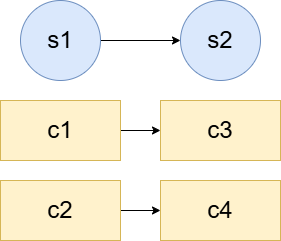
\includegraphics[width=5cm]{./img/treefuser-example-dgraph.png}
\subcaption{Dependence graph before fusion}
\label{fig:treefuser-example-3}
\end{subfigure}%
\begin{subfigure}{0.5\textwidth}
\centering
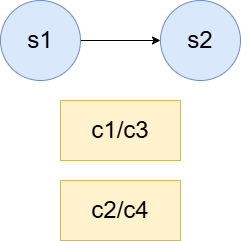
\includegraphics[width=4.3cm]{./img/treefuser-example-dgraph2.png}
\subcaption{Dependence graph after fusion}
\label{fig:treefuser-example-4}
\end{subfigure}

\begin{subfigure}{\textwidth}
\begin{lstlisting}[style = mystyle_grafter_example]
    fused_traversal(n, do_1, do_2)
      if do_1
        n.v = n.v + 1                   [s1]
      if do_2
        n.v = n.v * 2                   [s2]
      fused_traversal(n.l, do_1, do_2)  [c1/c3]
      fused_traversal(n.r, do_1, do_2)  [c2/c4]
\end{lstlisting}
\subcaption{Example resulting fused code}
\label{fig:treefuser-example-5}
\end{subfigure}
\caption{An example of the TreeFuser algorithm.}
\label{fig:treefuser-example}
\end{figure}

In \autoref{fig:treefuser-example-1}, the two functions are defined. Each function consists of three statements: the transformations (on lines 2 and 7, respectively), and the recursive calls for the traversals (lines 3 and 4, and lines 8 and 9). We will call the statements from the \texttt{increment} function \texttt{s1}, \texttt{c1}, and \texttt{c2}. The statements from the \texttt{multiply} function will be called \texttt{s2}, \texttt{c3}, and \texttt{c4}. Both \texttt{s1} and \texttt{s2} (the transformations) perform a read and write on \texttt{n.v}. The recursive calls traverse down into either \texttt{n.l} or \texttt{n.r}, and then execute the function they called on that node. That means they perform a read and write on either \texttt{n.l.v} or \texttt{n.r.v}, but also recursively continue to traverse down into the children of either \texttt{n.l} or \texttt{n.r}. Effectively, this constructs a regular expression that describes the reads and writes of these calls, as shown in \autoref{fig:treefuser-example-2}.

A dependence graph can be constructed based on the results of the dependency analysis by checking where two statements access the same location, with at least one of the statements being a write. For any such access intersection, an edge is added in the dependence graph between the two statements to maintain their relative ordering. The result of this is shown in \autoref{fig:treefuser-example-3}. In this case, there are only three edges.

The algorithm then attempts to merge nodes in the dependence graph, which represents traversal fusion. It is only legal to merge call nodes. These call nodes also have to, logically, traverse down into the same child to be able to be fused. This means a fusion of \texttt{c1} with \texttt{c3} is possible in this example, as well as a fusion of \texttt{c2} with \texttt{c4}. The resulting dependence graph is shown in \autoref{fig:treefuser-example-4}. Because this fusion has not resulted in any cycles in the dependence graph, it is also a legal fusion.

We will not discuss the final step (the synthesis of the fused traversal code) in detail here, but possible fused code that could be generated for this example has been included in \autoref{fig:treefuser-example-5}. In essence, a topological order for all statements is extracted from the dependence graph after fusion, and a function is then built from statements in that order. In this case, this does indeed result in a fused function that performs fewer total node visits than the unfused version, which might already be inferred from the fact that there are only two call nodes remaining instead of four.

An important benefit of both the TreeFuser and Grafter algorithms is that they support the concept of partial fusion, enabling many more fusion opportunities than algorithms that look only at opportunities for full fusion. Consider, for example, a scenario in which \texttt{c1} and \texttt{c3} could be fused in the previous example, but \texttt{c2} and \texttt{c4} could not. That implies that the traversals can be merged on the left children of a node, but not on the right children. This leads to a somewhat unusual fused traversal, but one that does perform fewer total node visits.

The most important difference between TreeFuser and Grafter, then, is that TreeFuser assumes trees are homogeneous (consist of only a single constructor). Grafter performs a more complex analysis that allows heterogeneous trees (multiple different constructors) to be analyzed, and also enables type-specific partial fusion. That means fusion cannot only be performed on some children but not on others, but also on some constructors but not on others. 

In addition, both TreeFuser and Grafter are formally proven to be sound, and thus provide a solid basis for a strategic programming traversal fusion algorithm. There are, however, also important differences between imperative and strategic programming and limitations of both algorithms that need to be addressed to achieve traversal fusion in strategic programming. The most important of these are:

\begin{itemize}
    \item In strategic programming, the transformations and traversals are explicitly separated, instead of incorporated into a single function that can be analyzed
    \item In strategic programming, traversal functions are not normally represented as functions that make recursive calls on individual children
    \item In strategic programming, transformations are not represented as statements, but rather as rewrite rules that make their reads and writes less explicit
    \item Neither algorithm supports conditionally made recursive calls, which are much more common in strategic programming
    \item Code synthesis must logically result in a strategic program, not an imperative one
    \item Strategies are definitionally generic, making support for heterogeneous trees unavoidable, and complicating most steps of the algorithm
\end{itemize}

In the next chapter, we will demonstrate a solution for traversal fusion in strategic programming based on a combination of both of these algorithms, and that incorporates new methods to work around the issues outlined above.

%And the fact that it's not really fusion of traversals but of recursive calls in a 'traversing function'... A method inspired by this for strategic programming, could that work?%

%If it does work, can we extract features of the rules for which it works, to have a way of sort of saying 'if your rules obey X, Y, Z constraints, you can fuse certain traversals generically like so' without necessarily specifying the rules completely? E.g. sequential topdown for rules that only look at direct children. Provable through \autocite{SakkaS017, SakkaSN019} method?%
% !TEX root = document.tex

\lstdefinestyle{mystyle_ex_stratego_program}{
language = Python,
morekeywords = {1, 2, r1, r2, Exp, E, Null, A, B, prog, Plus},
keywordstyle = [2]{\color{num_color}},
morekeywords = [2]{1, 2},
keywordstyle = [3]{\color{kw_alt}},
morekeywords = [3]{signature, sorts, constructors, Int, strategies, topdown, rules, add}
}
\lstdefinestyle{mystyle_automaton_pseudo}{
language = Python,
morekeywords = {Map, put, contains, get},
keywordstyle = \color{kw_alt},
keywordstyle = [2]{\color{magenta}},
morekeywords = [2]{Statement, Constructor, Automaton, automatonMap, constructAutomata, build, buildStatementAutomaton, getChild, addToStart, addTransition}
}
\lstdefinestyle{mystyle_fused_stratego}{
language = Python,
morekeywords = {r1, r2, Null, A, B, f_main, f_main_A, f_main_B, f_main_Null, f_0, f_0_A, f_0_B, f_0_Null, f_1, f_1_A, f_1_B, f_1_Null},
keywordstyle = [2]{\color{kw_alt}},
morekeywords = [2]{id}
}

\chapter{\label{chap:solution}A Traversal Fusion Algorithm for Strategic Programming}

In this chapter, we describe the algorithm that we have developed for generic traversal fusion in strategic programming. This algorithm predicts opportunities for traversal fusion by performing a dependency analysis on the program as a whole (i.e. its traversals and rewrite rules).

By analyzing the operations that rewrite rules perform, as well as how the traversals interact with this process, it is possible to construct a (partial) order that specifies which operations need to happen before others in the program. The algorithm then attempts to fuse together the recursive call operations that make up the traversals of the program. In case any two such statements can be fused without causing a dependency cycle, traversal fusion can be performed on those calls.

The algorithm consists of five main steps based on both the TreeFuser and Grafter algorithms \cite{SakkaS017, SakkaSN019}, each of which will be described in detail in the following. The steps are:
\begin{enumerate}
    \item Parsing and extracting the necessary information from the source program;
    \item Performing a dependency analysis on the rewrite rules and traversals;
    \item Building a dependence graph from the dependency analysis results;
    \item Finding fusion opportunities in the dependence graph;
    \item Synthesizing a program with fused traversals.
\end{enumerate}

\section{Soundness of Fusion with Dependency Analysis}
Before exploring the algorithm in more detail, we will touch on why the approach that predicts fusion opportunities using dependency analysis is sound. A thorough analysis of the soundness of this approach has been done, which identified two criteria that a sound fusion must satisfy: preservation of work and preservation of dependencies \cite{SakkaS017, SakkaSN019}. In short, the fused version of a program must perform exactly those operations on nodes that were performed in the original program, and if two operations have a dependency relation, they must be performed in the same order as in the original program.

Note that these criteria are true in general, regardless of the approach taken to fusion. The intuition here is that, if two operations on a node do not have a dependency relation, it cannot possibly matter for the final result in which order these operations are performed. Then, any program that performs the exact same operations while respecting all dependency relations must lead to the same result.

This, of course, logically leads to using dependency analysis to predict fusion opportunities, as it directly satisfies the dependency relation criterion. The other criterion is relatively easily satisfied by not touching the rewrite rules in our case.

\section{Information Extraction}
The most important pieces of information required from the source program are the outline of the program (i.e. which traversals are used and in which order), the definitions of the rewrite rules used in those traversals, as well as information about the constructors and their types.

In Stratego, this information is extracted using the standard parser for the language. The prototype implementation only supports a subset of the Stratego language and makes some assumptions about the format of the input program.

Specifically, we require:
\begin{itemize}
    \item A declaration of all sorts, and all constructors and their types
    \item Constructors to only be simple types using the declared sorts (e.g. no list types)
    \item A single main strategy called \texttt{prog} that consists of a sequence of calls to \texttt{all}, rule applications, calls to the built-in strategies \texttt{topdown} or \texttt{bottomup}, or calls to other strategies using only these features
    \item Rewrite rules to only perform pure rewrites without side effects (function calls are allowed)
\end{itemize}

These limitations will be discussed in more detail in \autoref{sec:limitations}, including an analysis of which limitations are inherent to the algorithm, and which limitations exist only due to time constraints, including suggestions on how to address them.

After extracting the necessary information, some processing is required before we continue to the next step. Note that what appears to be a single rewrite rule is actually a set of rewrite rules with the same label in Stratego, and a single label can consequently have an arbitrary number of definitions. The left-hand side of such a definition is a match statement (which could and usually does match on the constructor). This means the constructor changes which rewrite rules within a rewrite rule set are active. This has significant implications for the dependency analysis, because a ruleset could do something completely different on a different constructor. As such, each ruleset is separated into multiple virtual sets differentiated by the constructor in their left-hand side match statement for the dependency analysis.

An example of a program that can be analyzed using this algorithm has been included in \autoref{fig:ex-stratego-program}, and will also be used as an example throughout this chapter. This program does not compute anything useful, but serves as a good illustration of the possible different cases that can occur while executing the algorithm.

\begin{figure}
\begin{lstlisting}[style = mystyle_ex_stratego_program]
    signature
      sorts
        Exp

      constructors
        Null : Exp
        A : Exp * Exp * Int * Int -> Exp
        B : Exp * Int -> Exp

    strategies
      prog = topdown(r1); topdown(r2)

    rules
      r1 :
        Null() -> Null()
    
      r1 :
        A(l, r, a, b) -> A(l, r, (<add> (a, b)), b)

      r1 :
        B(c, v) -> B(c, (<add> (v, 1)))

      r2 :
        Null() -> Null()

      r2 :
        A(A(ll, lr, la, lb), r, a, b) -> A(A(ll, lr, la, lb), r, (<add> (a, la)), b)

      r2 :
        A(B(c, v), r, a, b) -> A(B(c, v), r, (<add> (a, v)), b)

      r2 :
        B(c, v) -> B(c, (<add> (v, 1)))
\end{lstlisting}

\caption{Example Stratego program to be analyzed.}
\label{fig:ex-stratego-program}
\end{figure}

\section{Dependency Analysis}
The dependency analysis determines the \textit{reads} and \textit{writes} made by all the rewrite rules. These terms refer to locations that are read from or written to by a rewrite rule, respectively. We give an exact definition in the context of strategic programming later on in this chapter.

After analyzing the rewrite rules, the dependency analysis determines the reads and writes of the recursive calls of a traversal. This is a necessary step in building the (partial) execution order of the program.

\subsection{Access Paths and Access Automata}
The dependency analysis makes use of access paths and access automata.

Access paths are a generic way of discussing locations relative to a certain node. The children of a node are numbered from left to right, starting from 0. Then, for example, the left child of a node with two children can be referred to with \texttt{n.0}, and its right child with \texttt{n.1} (with \texttt{n} always referring to the current node). Access paths are, in essence, regular expressions. Further descendants can thus easily be pointed to with \texttt{n.0.0}, \texttt{n.0.1}, and so on. Furthermore, \texttt{n(.0)*} could point to \texttt{n}, \texttt{n.0}, \texttt{n.0.0}, etc. When constructing the reads and writes of traversals, these paths will become more complex, and it is easier to construct them as their equivalent automata. These are called access automata.

\subsection{Type-Specific Analysis}
In the dependency analysis, the algorithm cannot make any assumptions about the structure of the input data other than the information gathered from the constructor definitions. And because strategies are generic, it is not possible to know the type of the node they will be called on, the types of its children, or even its number of children. In addition, note again that rewrite rules are actually sets that may have multiple definitions (differentiated by the constructor of the node they are executed on). Consequently, the dependency analysis has to be performed separately for every possible constructor.

The logical conclusion of the previous statement is that it may be possible to fuse certain strategies when executing on one constructor, but not on another. This is the type-specific partial fusion discussed in \autoref{sec:towards-a-solution}.

Note that this type-specific analysis, in most cases, makes the analysis more complex than simpler. Consider the \texttt{A} and \texttt{B} constructors in \autoref{fig:ex-stratego-program}. They both are constructors of the \texttt{Exp} sort, and also each have children of the \texttt{Exp} sort. This means they are mutually recursive and their dependency analyses, while performed separately, may still need to interact with each other.

\subsection{Rewrite rules}
Determining the reads and writes of the rewrite rules is required to determine the reads and writes of the traversals. Rewrite rules in strategic languages do not read and write to locations in the same way as might occur in an imperative language. The notions of reading and writing will be defined as follows:

A rewrite rule has a left-hand side, and a right-hand side. On the left, it performs a match to determine whether the rule applies to the current node. This can be considered to be a read, because the necessary terms need to be read to determine whether the match applies to this node. A match statement does not necessarily always read all the children of a node. For example, consider the following rule:

\begin{lstlisting}[style = mystyle_ex_stratego_program]
    Plus(left, right) -> Plus(left, 1)
\end{lstlisting}

Despite both \texttt{left} and \texttt{right} being named in this rule, neither is ever read. Nothing happens to \texttt{left}, and \texttt{right} is always overwritten, regardless of what its value was.

In contrast, a rule such as
\begin{lstlisting}[style = mystyle_ex_stratego_program]
    Plus(left, 1) -> Plus(left, 2)
\end{lstlisting}

Does perform a read on the child that was called \texttt{right} in the previous rule (i.e. the location \texttt{n.1}). It has to be read to check whether its value is \texttt{1}, in order to determine whether the rewrite rule applies.

Then, if a location is not assigned a variable, but instead is matched on with a concrete value, it is \textit{always} read. If a location \textit{is} assigned a variable, it may or may not be read. Consider this rule:
\begin{lstlisting}[style = mystyle_ex_stratego_program]
    Plus(left, right) -> Plus(right, right)
\end{lstlisting}

Here, the location \texttt{n.1} \textbf{is} read, because its value has to be copied to \texttt{n.0}. The notion of reading in the context of a dependency analysis does include copying: while it is theoretically possible to copy a value in memory without reading its contents, this still introduces a read dependency. That is to say, if a later statement were to alter the value in \texttt{n.1}, it would \textbf{not} be legal to move that statement before this one in the program.

From this, the following concrete rules are derived to determine whether a location is read:
\begin{enumerate}
    \item If a location \textbf{is matched on with a concrete value}, it is always read.
    \item Otherwise, if a location is assigned a variable, it is read \textbf{only} if that variable occurs in a different location on the right-hand side.
\end{enumerate}

Writes are simpler to analyze: a location is written to if and only if its value on the right-hand side is not equal to its value on the left-hand side.

Finally, the algorithm also supports wildcards and calls to pure functions in rewrite rules.

Wildcards can only occur on the left-hand side. Locations matched with a wildcard are never read, but always written to.

Function calls can only occur on the right-hand side. They always write to their location. Their reads are a union of all their function arguments. It is legal to ignore what the function actually does internally because it is pure: for the purposes of the dependency analysis, calling a function is identical to writing a tuple of all the function arguments to a location.

\subsection{Correctly Constructing Automata}
The rules in the previous section define what reads and writes are in the context of rewrite rules. However, some additional rules are necessary to correctly construct access automata for the dependency analysis.

First, in the case of a rewrite ruleset with multiple definitions, the reads and writes of all definitions that apply to the constructor currently being analyzed can be combined. We use an automaton union algorithm for this.

Second, and most importantly, all prefixes of the read and write automata constructed also need to be considered:

\begin{itemize}
    \item For read automata, every prefix is also read. That means that every state except the initial state is an accept state.
    \item For write automata, only the final state is an accept state. However, all prefixes are read, and as such should be added to the rewrite rule's read automaton.
\end{itemize}

Equivalently, we could say that both read and write automata always read all their prefixes. The intuitive reason for this is that these prefixes represent the parent nodes of the location being referenced with the automaton, and writing to one of the parents should cause a dependency conflict with the child as well.

It is perhaps better illustrated with an example: two rewrite rules operating on a binary tree as seen below.

\begin{lstlisting}[style = mystyle_ex_stratego_program]
    r1: E(E(ll, lr), r) -> E(E(ll + 1, lr), r)
    r2: E(_, r) -> E(r, r)
\end{lstlisting}

The first reads and writes to location \texttt{n.0.0}, while the second writes to \texttt{n.0}. Without considering prefixes, these two rewrite rules would not conflict, and the second could theoretically be moved in front of the first. However, that should be illegal: the write to \texttt{n.0} implicitly overwrites the value in \texttt{n.0.0}. In the original execution order, that would be the final value stored in the node. If the rewrite rules were swapped, that value would be incremented by one.

\subsection{Traversals}
With the reads and writes of the rewrite rules determined, it becomes possible to define the reads and writes of the traversals. The core idea is to analyze traversals as recursive functions, consisting of statements that apply rewrite rules, and calls that call a function on one or multiple child nodes. We are now interested in determining the reads and writes of these calls.

The reads and writes for calls must be analyzed in a type-partial way. So, the algorithm considers every constructor and analyzes the reads and writes of a call, given that it is executed on a node of that constructor. The \texttt{all} function (that executes it argument on every child of a node) is split into multiple individual calls for every child (which is now possible because we know how many children this constructor has).

The actual reads and writes of such a call, then, are defined recursively. Consider, for example, \texttt{r1} from the example given in \autoref{fig:ex-stratego-program}, executing on a node with constructor \texttt{B}. This rule both reads and writes to the location \texttt{n.1}. Ignoring the possibility of a child with constructor \texttt{A} for now, executing this rule \texttt{topdown} would cause it to be applied recursively on the left child. This means the call to the left child reads and writes \texttt{n.0.1}, \texttt{n.0.0.1}, etc. This is precisely what is needed for the dependency analysis.

If we do consider the possibility for a child with constructor \texttt{A}, these access paths quickly become more complex. The algorithm therefore is based on constructing access automata. 

\autoref{fig:traversal-dependency-pseudocode} shows the pseudocode of the algorithm that constructs the dependency automata.

This algorithm recursively constructs a set of automata representing the read and write dependencies for every statement in the program executing on every possible constructor. These automata are mutually recursive, but the algorithm is guaranteed to terminate because if an automaton has already been constructed for a certain statement executing on a certain constructor, a reference to that automaton is simply inserted instead of creating a new one.

\subsection{Example Construction}
To illustrate the read/write analysis and the construction of the read/write automata more clearly, we will use the example program from \autoref{fig:ex-stratego-program}. The automata will be built up step by step in \autoref{fig:ex-automata}. We will build the automata per constructor, starting with \texttt{Null}.

\texttt{Null} has no children, which means it does not perform calls. There are only two statements to analyze: the one representing the application of \texttt{r1}, and the one representing the application of \texttt{r2}. Neither \texttt{r1} nor \texttt{r2} perform reads or writes on \texttt{Null}. As such, both statements generate an automaton with a single non-accepting start state with no edges (equivalent to an empty automaton).

Next, we look at the constructor \texttt{B}. It does have a single child on which a traversal can be called, and the rewrite rules do perform an operation on nodes with this constructor. This means there are four statements in total to analyze: one for each rewrite rule application, one call statement (on the only child) from the first traversal, and one call from the second traversal. We label the first call \texttt{c0}, and the second \texttt{c1}. First, we note that \texttt{r1} and \texttt{r2} are equivalent for \texttt{B}. They perform a single read and write, on \texttt{n.1}. We have now arrived at the situation seen in \autoref{fig:r_w_2}. Next, we will look at the call statements. There are two functions that can be called, corresponding to the two traversals. These functions consist of the rewrite rule application statements, as well as the traversal call statements. \texttt{B}'s child is of type \texttt{Exp}, which means its constructor can be either \texttt{A}, \texttt{B}, or \texttt{Null}.

We start with a single non-accepting start state for each call statement. In case the child constructor is \texttt{Null} or \texttt{B}, the following happens: the algorithm sees that the automata for all statements in the called function on that constructor have already been generated (the automaton for the call on \texttt{B} is a reference to the one currently being constructed). \texttt{B}'s child lives at index \texttt{0}, and as such edges labeled with \texttt{0} are added, pointing to all the automata for every statement in the function being called. This is illustrated in \autoref{fig:r_w_3}.

We also have to consider the case in which \texttt{B}'s child has constructor \texttt{A}. This will trigger the dependency analysis for the \texttt{A} constructor. It has more statements because it has two children instead of one: there are still two rewrite rule application statements, but there are now four call statements (one per child per traversal). \texttt{c0} is the call on the left child from the first traversal, \texttt{c1} the call on the right child from the first traversal. \texttt{c2} and \texttt{c3} are the calls on the left and right children respectively from the second traversal. \texttt{r1} on \texttt{A} reads \texttt{n.2} and \texttt{n.3}, and writes to \texttt{n.2}. \texttt{r2} also writes to \texttt{n.2}, but reads \texttt{n.0}, \texttt{n.0.1}, \texttt{n.0.2}, and \texttt{n.2}. This creates the automata seen in \autoref{fig:r_w_4}.

\texttt{A}'s children are also of type \texttt{Exp}, and as such can have constructor \texttt{A}, \texttt{B}, or \texttt{Null}. All other automata have now been constructed, so the insertion of the reference edges proceeds in the same way. Edges from \texttt{B}'s calls pointing to \texttt{A} can now also be inserted. The final construction is seen in \autoref{fig:r_w_5}.

\begin{figure}
\centering
\begin{subfigure}{0.45\textwidth}
\centering
\raisebox{39pt}{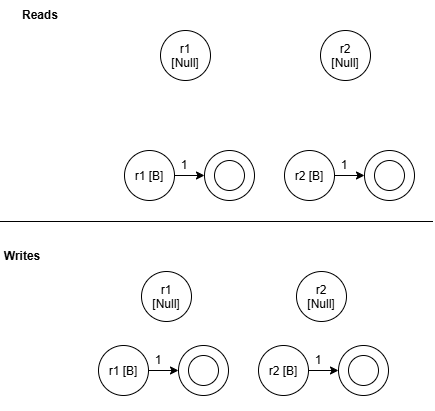
\includegraphics[width=\linewidth]{./img/r_w_2.png}}
\subcaption{Step 1.}
\label{fig:r_w_2}
\end{subfigure}%
\begin{subfigure}{0.45\textwidth}
\centering
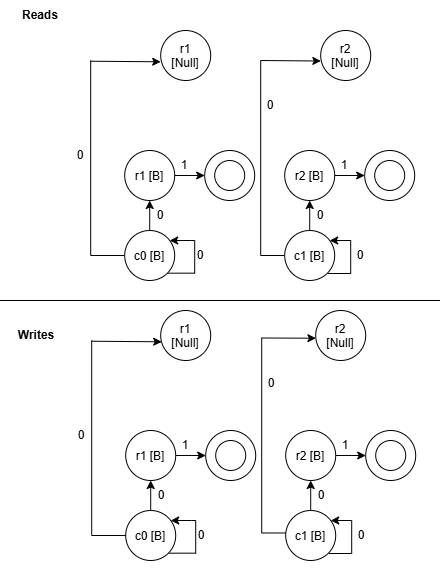
\includegraphics[width=\linewidth]{./img/r_w_3.png}
\subcaption{Step 2.}
\label{fig:r_w_3}
\end{subfigure}

\begin{subfigure}{0.45\textwidth}
\centering
\raisebox{25pt}{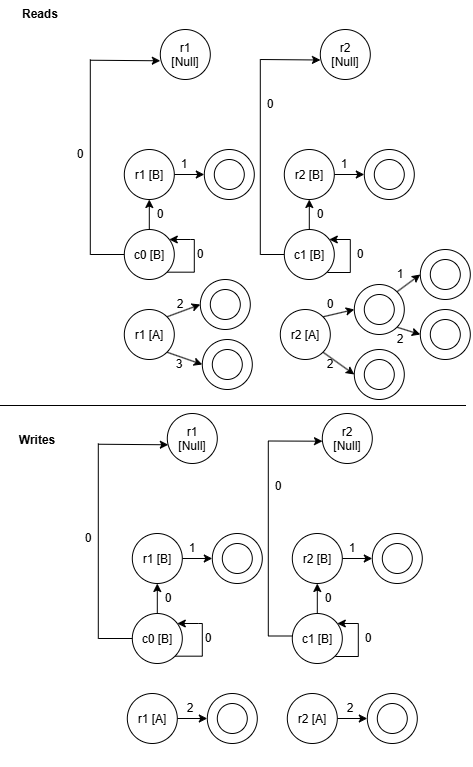
\includegraphics[width=\linewidth]{./img/r_w_4.png}}
\subcaption{Step 3.}
\label{fig:r_w_4}
\end{subfigure}%
\begin{subfigure}{0.45\textwidth}
\centering
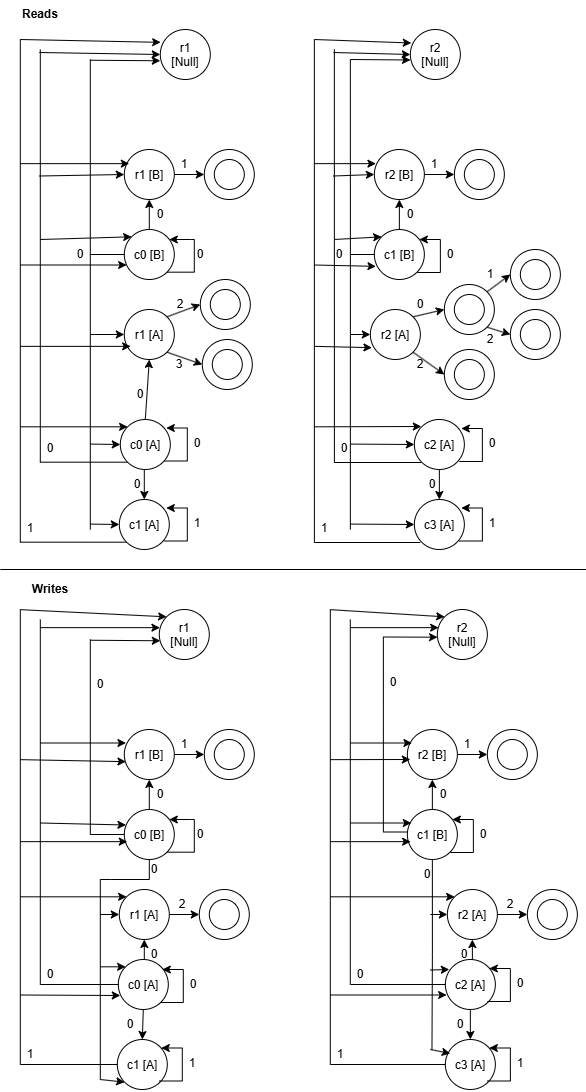
\includegraphics[width=\linewidth]{./img/r_w_5.png}
\subcaption{Step 4.}
\label{fig:r_w_5}
\end{subfigure}

\caption{Read/write automaton construction for the example program in \autoref{fig:ex-stratego-program}.}
\label{fig:ex-automata}
\end{figure}

\begin{figure}
\begin{lstlisting}[style = mystyle_automaton_pseudo]
Map<(Statement, Constructor) -> Automaton> automatonMap;

constructAutomata():
  for c in possible constructors:
    for f in functions:
      build(c, f)

build(c, f):
  for s in f.statements:
    if s is rewrite rule:
      resultAutomaton = buildStatementAutomaton(s, c)
      automatonMap.put((s, c) -> resultAutomaton)
      return resultAutomaton
    else if s is call:
      child = c.getChild(s.idx)
      resultAutomaton = null;
      for childC in child.possibleConstructors:
        automaton = null;
        if automatonMap.contains((s, c)):
          automaton = automatonMap.get((s, c))
        else:
          automaton = build(childC, s.calledFunction)
        resultAutomaton = addToStart(resultAutomaton, s.idx, automaton)
      automatonMap.put((s, c) -> resultAutomaton)
      return resultAutomaton

addToStart(a1, c, a2):
  a1.startState.addTransition(c, a2.startState)
\end{lstlisting}

\caption{Pseudocode of the traversal dependency analysis algorithm.}
\label{fig:traversal-dependency-pseudocode}
\end{figure}
%With the reads and writes of the rewrite rules determined, we can now also define the reads and writes of the traversals. Essentially, the idea is that analyzing these traversals as recursive functions constructs an access path that is a regular expression. For example, consider the following example of a binary tree and a simple traversal rule that increments a stored value inside a node.%

%\begin{lstlisting}
%    rule:
%      E(left, right, val) -> E(left, right, Plus(val, 1))
%\end{lstlisting}

%We analyze the reads and writes of the rewrite rule using the method described in the previous section. Clearly the only write is to the location \texttt{n.2}, as that is the only location that is changed by the rewrite rule. The only read is also on \texttt{n.2} - note that the variable \texttt{val} does indeed appear in a different location on the right-hand side of the rule (\texttt{n.2.0} instead of \texttt{n.2}).%

%Then, if we were to perform a topdown traversal with this rule, consider what would happen. We execute the rule on the current node (reading and writing to \texttt{n.2}), then go into either the left or right child (\texttt{n.0} or \texttt{n.1}), then execute the rule on those children, and continue into their children, etc.%

%This means the reads and writes performed by the traversal look like this: \texttt{n.2}, \texttt{n.0.2}, \texttt{n.1.2}, \texttt{n.0.0.2}, \texttt{n.0.1.2}, ...%

%Or, in a regular expression, \texttt{n(.0|.1)*.2}%

%Now, we consider the application of the rule to the current node to not be part of the recursive calls for the traversal, and analyze the traversal down into each of the children separately. This means that, in this example of a binary tree, a topdown traversal generates two calls with reads and writes of \texttt{n.0(.0|.1)*.2} and \texttt{n.1(.0|.1)*.2}.%

\section{Building the Dependence Graph}
After performing the dependency analysis, the rules and traversals are analyzed in program order. The notion of program order is not very strictly defined in a strategic language. Whereas one can simply read a program in order in an imperative language, rewrite rules and traversals can be more abstractly defined. In order to overcome this problem, we analyze rewrite rules as single statements that perform all their read and write operations at the same time. This means our fusion algorithm will never pull rewrite rules apart. It is theoretically possible that splitting a rewrite rule into multiple statements could increase fusion opportunities, simply by being more permissive in the program order, but this would also further complicate the algorithm. For traversals, the program order is defined simply as all the recursive calls executed in order. For \texttt{all}, we assume the calls to the children are made left-to-right.

%As mentioned before, the traversals have to be analyzed as recursive functions. For \texttt{topdown}, it is relatively easy to extract a program order from its concrete definition. It executes the rewrite rule, and then the calls to the children of the current node happen in sequence. For more complex traversals, defining a program order may be more difficult. For example, it is not possible to directly incorporate conditional calls. \textit{We analyze traversals like these like regular topdown/bottmup traversals, but have to insert and alter rewrite rules to keep track of whether the rewrite rule has been applied to a node yet, and to prevent further applications of the rule if it has(?)}.%

With a program order defined, a graph is created for every type of constructor. In every graph, a node is created for every statement (rewrite rule) and every recursive call. For every node, we check whether its read and write dependencies interfere with a node that follows it in the program order. Interference in this case means an intersection of the access path automata of the nodes, with at least one of those automata being a write automaton. If there is such interference, an edge is added between those nodes in the dependence graph.

Calls that descend into children that are of primitive (built-in) Stratego types (such as \texttt{Int}) are automatically ignored in the prototype. While the algorithm can easily deal with these calls, ignoring them drastically improves performance by reducing the search space for fusion opportunities. It is a legal optimization under the condition that no rewrite rule directly matches on such a primitive type.

At this stage, nearly all information about what the program actually does has been erased. However, every node is annotated with the traversal that it originated from, and call nodes also include information on which child of the parent they call. Retaining this information is important for finding correct fusion opportunities, because call nodes operating on different children can, logically, never be merged legally.

For the example in \autoref{fig:ex-stratego-program}, three graphs are created. They are all displayed in \autoref{fig:ex-stratego-program-d-graphs}. The graph for the \texttt{Null} constructor is the simplest: because \texttt{Null} does not have any children, there are no call nodes. It only contains the two statement nodes (\texttt{s0} and \texttt{s1}) representing the rewrite rule applications. The graphs for \texttt{A} and \texttt{B} do contain call nodes in addition to those same statement nodes. Note that the call nodes that descend into the primitive type \texttt{Int} are ignored. This means that the graph for \texttt{A} contains two call nodes per traversal representing the calls that traverse into its non-primitive children. That means there are four in total: \textbf{c0} and \texttt{c1} originate from the first traversal, while \texttt{c2} and \texttt{c3} come from the second. These are arranged by column (the left column contains all nodes from the first traversal, while the right column contains all nodes from the second). The graph for \texttt{B} contains one call node per traversal (so, two in total).

The edges in these graphs represent dependency relations: the dependency analysis has determined that these nodes' automata conflict in some way, constructing a partial order between them. It is possible to verify these edges using the automata created in \autoref{fig:ex-automata}. For every edge, take the start and end nodes. Then, find their corresponding automaton states (\texttt{s0} and \texttt{s1} correspond to states named \texttt{r1} and \texttt{r2}, respectively). There will be a state in the read automaton as well as one in the write automaton for that node. Now, there must exist a pair of states corresponding to these nodes (with at least one of the states being in the write automaton) that intersects on a path to an accept state.

As an example, take \texttt{c0} and \texttt{c1} on \texttt{B}. We reference \autoref{fig:r_w_3} for simplicity. Take \texttt{c0} in the read automaton, \texttt{c1} in the write automaton. Follow the path \texttt{0 -> 1}. This path leads to an accept state for both automata, indicating a conflict between these two statements.

\begin{figure}
\begin{subfigure}{0.33\textwidth}
\centering
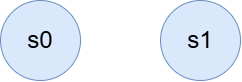
\includegraphics[width=4cm]{./img/ex-stratego-prog-d-1.png}
\subcaption{Dependence graph for \texttt{Null}.}
\label{fig:ex-stratego-program-d-graphs-1}
\end{subfigure}%
\begin{subfigure}{0.33\textwidth}
\centering
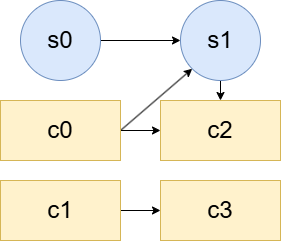
\includegraphics[width=4cm]{./img/ex-stratego-prog-d-3.png}
\subcaption{Dependence graph for \texttt{A}.}
\label{fig:ex-stratego-program-d-graphs-2}
\end{subfigure}%
\begin{subfigure}{0.33\textwidth}
\centering
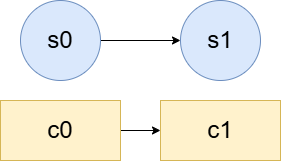
\includegraphics[width=4cm]{./img/ex-stratego-prog-d-2.png}
\subcaption{Dependence graph for \texttt{B}.}
\label{fig:ex-stratego-program-d-graphs-3}
\end{subfigure}

\caption{Dependence graphs of the example Stratego program in \autoref{fig:ex-stratego-program}.}
\label{fig:ex-stratego-program-d-graphs}
\end{figure}

\section{Finding Fusion Opportunities}
\label{sec:finding-fusion-opportunities}
For every call node in the dependence graph, the algorithm checks whether it can be merged with another call. It does this by merging their nodes in the graph. If this does not cause a cycle, the fusion is legal. Edges between the nodes being merged are simply removed and do not cause a self-loop.

As an aside, ignoring self-loops created in this manner makes it legal to fuse two call nodes that have a dependency relation without explicitly preserving their relative ordering. The reason this is legal is because their relative ordering must be preserved through dependency edges between statement nodes\footnote{We refer to the TreeFuser paper for a formal proof of the soundness of fusion\cite{SakkaS017}}. Of course, the relative ordering to all other nodes is always preserved when fusing.

We can only attempt to fuse calls that descend into the same child. For example, it is not legal to fuse a call that goes into the left child of a binary tree from one traversal with a call that descends into the right child from another traversal. Fusion can also only happen across different traversals, so the algorithm never attempts to fuse two calls that originate from the same traversal function.

Note that a single program may have multiple opportunities for fusion. Some fusions may exclude other opportunities, while some may be able to be combined. The algorithm attempts to exhaustively explore every possible combination of fusions, but this may quickly become prohibitively expensive for larger programs. 

Returning to the example dependence graphs shown in \autoref{fig:ex-stratego-program-d-graphs}, fusion proceeds as follows. The graph for \texttt{Null} does not contain any calls and as such there are no fusion opportunities. The graph for \texttt{B} has two calls that are from different traversals and traverse down into the same child. The algorithm attempts to fuse them. This results in the graph shown in \autoref{fig:ex-stratego-program-d-graphs-fused-1}, which does not contain a cycle. This means that the fusion is legal.

The graph for \texttt{A} contains four calls. There are two fusion opportunities: \texttt{c0} with \texttt{c2}, and \texttt{c1} with \texttt{c3}. The latter is a legal fusion and the resulting graph is shown in \autoref{fig:ex-stratego-program-d-graphs-fused-2}. 

The algorithm will also attempt to fuse \texttt{c0} and \texttt{c2}. However, this results in the graph shown in \autoref{fig:ex-stratego-program-d-graphs-fused-3}, which contains a dependency cycle. That means that this particular fusion is not legal.

\begin{figure}
\begin{subfigure}{0.33\textwidth}
\centering
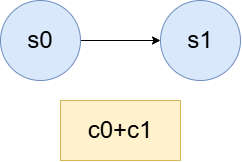
\includegraphics[width=4cm]{./img/ex-stratego-prog-d-2-fuse.png}
\subcaption{Fused graph for \texttt{B}.}
\label{fig:ex-stratego-program-d-graphs-fused-1}
\end{subfigure}%
\begin{subfigure}{0.33\textwidth}
\centering
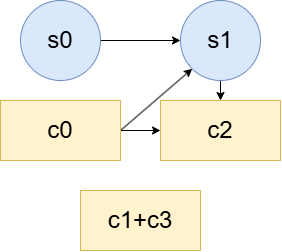
\includegraphics[width=4cm]{./img/ex-stratego-prog-d-3-fuse.png}
\subcaption{Fused graph for \texttt{A}.}
\label{fig:ex-stratego-program-d-graphs-fused-2}
\end{subfigure}%
\begin{subfigure}{0.33\textwidth}
\centering
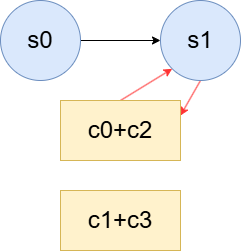
\includegraphics[width=4cm]{./img/ex-stratego-prog-d-3-fuse-illegal.png}
\subcaption{Illegal fused graph for \texttt{A}.}
\label{fig:ex-stratego-program-d-graphs-fused-3}
\end{subfigure}

\caption{Fused dependence graphs of the example Stratego program in \autoref{fig:ex-stratego-program} and \autoref{fig:ex-stratego-program-d-graphs}.}
\label{fig:ex-stratego-program-d-graphs-fused}
\end{figure}

\section{Fused Traversal Synthesis}
If the dependency analysis predicts one or multiple fusions, this will be evident from the fused nodes appearing in the dependence graph(s). However, these graphs need to be turned back into code that can execute the fused traversal.

The first step is to determine a new execution order. For every dependence graph, the algorithm places all the nodes in topological order based on the dependency edges present. This is always possible because the graph is guaranteed to be acyclic. Each graph may have a different number of nodes and a different resulting topological order.

As an aside, note that information about the original program order is ignored. This means that, even if the algorithm was not able to perform any fusion, the synthesized program may produce a different execution order. For example, it may be legal to change a top-down traversal to a bottom-up traversal in some cases. This is a feature of the algorithm, and it may be possible to use heuristics to prefer certain execution orders over others. In the prototype algorithm, we simply pick an arbitrary topological order without preference.

From the fused example graphs in \autoref{fig:ex-stratego-program-d-graphs-fused}, we get the following topological orders:
\begin{lstlisting}[style = mystyle_fused_stratego]
    Null : s0 -> s1
    A : s0 -> c0 -> c1+c3 -> s1 -> c2
    B : s0 -> c0+c1 -> s1
\end{lstlisting}

The algorithm first generates a \texttt{main} function that performs a match\footnote{\label{note-match-cong}Refer to \autoref{sec:additional-stratego-syntax} for an explanation of matches and congruences} on the current constructor, and calls a \texttt{main} function specialized to that constructor. For this example, it looks like this:
\begin{lstlisting}[style = mystyle_fused_stratego]
    f_main = ?A(_, _, _, _) < f_main_A + ?B(_, _) < f_main_B + ?Null() < f_main_Null + id
\end{lstlisting}

The algorithm then generates these \texttt{main} functions for every constructor, in which all statements from that constructor's topological order are inserted in order. Rewrite rule statements are inserted as invocations of the rule. Calls are inserted as a match on the constructor, with a function call then invoked on the correct child. The function we call also needs to be generated. To do this, we need the child and traversal annotations present on these nodes.

For example, when looking at the topological order for the \texttt{A} constructor in this example, the call \texttt{c0} is a call on the first child, originating from the first traversal. \texttt{c1 + c3} is a call on the second child, originating from both the first and second traversals (that is, from all traversals). Then, these statements together will be translated into the following Stratego code\footnote{See \ref{note-match-cong}}:
\begin{lstlisting}[style = mystyle_fused_stratego]
    A(f_0, f_main, id, id)
\end{lstlisting}

\texttt{f$\_$main} already exists and will select the correct \texttt{main} function for the constructor that the child happens to be. \texttt{f$\_$0} will have to be generated. It will also be a selector function that performs matches on the constructor, to then invoke the correct \texttt{f$\_$0} for the constructor in question. It looks like this:

\begin{lstlisting}[style = mystyle_fused_stratego]
    f_0 = ?A(_, _, _, _) < f_0_A + ?B(_, _) < f_0_B + ?Null() < f_0_Null + id
\end{lstlisting}

Generating these type-specialized functions is similar to generating the type-specified \texttt{f$\_$main} functions. The difference is that now only statements that originate from one of the selected traversals are inserted. For \texttt{f$\_$0}, that means we ignore all statements that do not originate from the first traversal. For \texttt{A}, that means \texttt{s1} and \texttt{c2} are ignored. \texttt{c1+c3} is inserted because it originates from both the first and second traversal. However, its part originating from the second traversal \textit{is} ignored. Whereas normally this call would generate a call to \texttt{f$\_$main}, it now also generates a call to \texttt{f$\_$0}. Then, we have

\begin{lstlisting}[style = mystyle_fused_stratego]
    f_0_A = r1; A(f_0, f_0, id, id)
\end{lstlisting}

The full synthesized code for this example is displayed in \autoref{fig:ex-stratego-program-fused-code}.

\begin{figure}
\begin{lstlisting}[style = mystyle_fused_stratego]
f_main = ?A(_, _, _, _) < f_main_A + ?B(_, _) < f_main_B + ?Null() < f_main_Null + id
f_0 = ?A(_, _, _, _) < f_0_A + ?B(_, _) < f_0_B + ?Null() < f_0_Null + id
f_1 = ?A(_, _, _, _) < f_1_A + ?B(_, _) < f_1_B + ?Null() < f_1_Null + id

f_main_A = r1; A(f_0, f_main, id, id); r2; A(f_1, id, id, id)
f_main_B = r1; B(f_main, id); r2
f_main_Null = r1; r2

f_1_A = A(id, f_1, id, id); r2; A(f_1, id, id, id)
f_1_B = B(f_1, id); r2
f_1_Null = r2

f_0_A = r1; A(f_0, f_0, id, id)
f_0_B = r1; B(f_0, id)
f_0_Null = r1
\end{lstlisting}

\caption{Synthesized fused code for the example Stratego program of \autoref{fig:ex-stratego-program}.}
\label{fig:ex-stratego-program-fused-code}
\end{figure}


\section{Limitations}
\label{sec:limitations}
In this section, we will discuss the limitations of our algorithm and the POC implementation in more detail.

First, and most importantly, we note that the algorithm cannot find all possible fusion opportunities. This is an inherent limitation of the algorithm: checking whether a fusion is legal using dependency analysis is sound but incomplete. In other words, if a fusion is illegal, there must be a dependency violation, but if there is a dependency violation, a fusion is not necessarily illegal. This means that the algorithm will never fuse something illegally, but it may not fuse all programs that can be fused. A more sophisticated dependency analysis could theoretically find more possibilities, but it cannot avoid the fact that a dependency violation does not always imply a fusion is illegal.

In contrast, there are a few limitations that exist only in the POC implementation of the algorithm. This does not necessarily imply they are easy to implement, but it is certainly possible to do so in theory. These are, in no particular order: constraints on constructor types (e.g. lack of list types), lack of support for side effects, constraints on the structure of the input program, required type declarations, and the lack of support for conditional traversals. We will discuss for each of these limitations in short how it might be addressed.

The constraints on constructor types are relatively straightforward to address. It is simply a matter of information extraction from the source program. Of course, the dependency analysis will also have to be updated to support list types, but it would not require any fundamental changes to the algorithm.

The lack of support for side effects is more complex. Of course, the algorithm would have to be able to correctly identify side effects. If those can be extracted from the source program, there would also have to be some more thorough changes to the dependency analysis algorithm. Side effects may have to be analyzed as reads and writes to global locations.

The constraints on the structure of the input program come down mostly to a matter of information extraction. However, it is important to remember that allowing for more complex input programs may also complicate code synthesis after fusion. It is important that no critical information about the structure of the program is lost, so that the program can be correctly synthesized back together in the end.

The required type declarations are an interesting limitation. It may be possible in theory to infer types for all constructors, removing the need for an explicit declaration. However, if this inference is less strict, some fusion opportunities may be lost.

Finally, the lack of support for conditional traversals is mostly a matter of code synthesis. Conditional traversals can be simulated with unconditional calls that immediately return\cite{SakkaSN019}. Again, it is important to keep in mind that there needs to be support for this in terms of information extraction (and retention throughout dependency analysis). However, if this can be done, the challenge is mostly a matter of synthesizing a correct program.
% !TEX root = document.tex

\chapter{\label{chap:evaluation}Evaluation}

In this chapter, we evaluate the algorithm for traversal fusion in strategic languages developed in the previous chapter. A proof-of-concept implementation that operates on a subset of Stratego has been created. This implementation is run on a synthetic program transformation benchmark that mimics real-world usage, as well as a benchmark simulating a best-case scenario for fusion. The evaluation aims to determine whether traversal fusion works at all in strategic languages, as well as to determine its effect on program runtime and memory usage.

\section{Benchmark Environment}
The benchmarks are run on the following machine:
\begin{itemize}
    \item \textbf{OS:} Windows 11 23H2 (22631.6199)
    \item \textbf{CPU:} Intel Core i7-9750H (6 cores, 2.6 GHz)
    \item \textbf{RAM:} 16 GB DDR4-2666
\end{itemize}

Benchmarks are run in Java using the Java Microbenchmark Harness (JMH). We use it to measure the elapsed program runtime and overall memory usage. In addition, JMH manages, among other things, Java Virtual Machine (JVM) warm-up, repeated runs, and result collection. Finally, a Python script is used to process the results and generate visualizations.

For all benchmarks, JMH has been configured to perform five warm-up runs, after which runtimes stabilize. After that, a series of measured runs is performed (normally ten, unless otherwise mentioned). In the resulting graphs, we use the mean of these ten runs, while the error bars represent one standard deviation.

\section{Benchmark Design}
It is important to design a benchmark that reflects real-world applications of strategic programming languages, because the number of fusion opportunities can differ significantly between different programs. The number of fusion opportunities, of course, directly influences the effectiveness of the traversal fusion optimization. The benchmark created for this evaluation performs several program transformations on a render tree for a custom web design language. This is a relevant real-world use case for strategic programming languages. Furthermore, the benchmark is based on a benchmark used as part of the evaluation for Grafter (the algorithm our solution is also based on), in which it was also selected for its real-world relevance \cite{SakkaSN019}. This also allows for a direct comparison between the effectiveness of our algorithm for strategic programming languages and the algorithm for imperative languages.

In addition to this render tree benchmark, a smaller benchmark simulating a best-case scenario for fusion has also been created. This benchmark consists of a simple binary tree of integers on which two top-down traversals are performed. These traversals can be fully fused into a single top-down traversal.

In the following section, the render tree and the transformations applied to it in the benchmarks will be explained in more detail. The actual Stratego implementation will differ slightly from this explanation in some cases. For example, there are more constructors that contain more fields, and the rewrite rulesets have more definitions. In most cases, these changes were made to work around limitations of the supported subset of Stratego. These implementation details are not relevant for understanding the benchmark and the results.

\subsection{Render Tree and Transformations}
The render tree used in this benchmark is, in essence, an abstract syntax tree representing the structure of a (simple) web page. Pages can have containers that contain elements such as text boxes or images. \autoref{fig:benchmark-render-tree-layout} shows the possible constructors for the render tree and how they relate in more detail. Note that the constructors \texttt{HorizontalContainer} and \texttt{VerticalContainer} are mutually recursive, allowing for complex nested render trees to be created.

The benchmark input size is measured in a number of pages. Every page is an identical sample page that contains each possible type of element (see \autoref{fig:benchmark-render-tree-sample-page}). This sample page is identical to the one used in the Grafter evaluation.

\begin{figure}
\centering
\begin{subfigure}{0.7\textwidth}
\centering
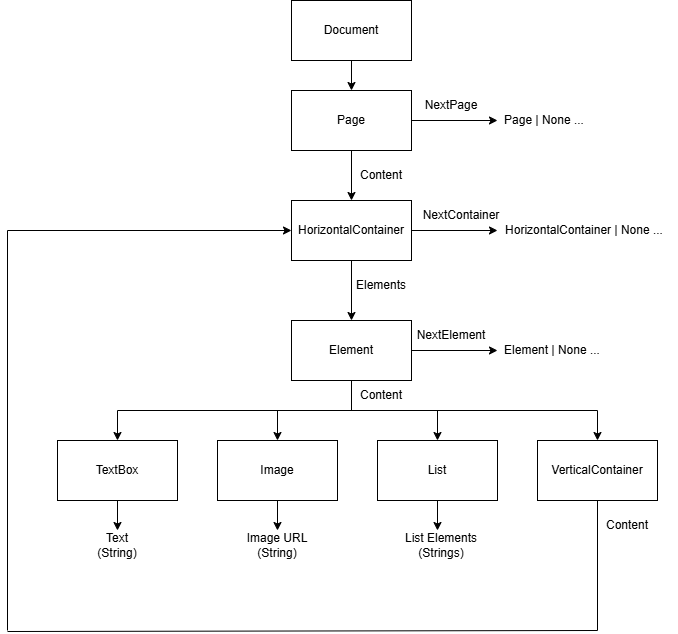
\includegraphics[width=\textwidth]{./img/benchmark-render-tree-layout.png}
\caption{Class layout of the render tree used in the evaluation.}
\label{fig:benchmark-render-tree-layout}
\end{subfigure}

\begin{subfigure}{0.7\textwidth}
\centering
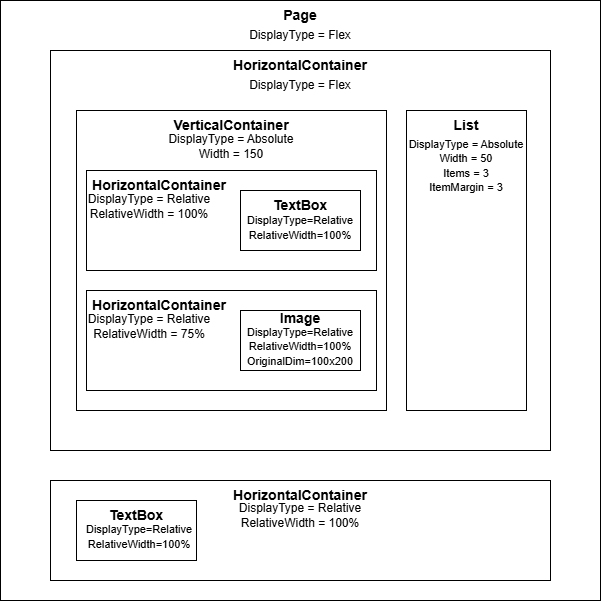
\includegraphics[width=\textwidth]{./img/samplepage.png}
\caption{Sample page used in the render tree benchmark.}
\label{fig:benchmark-render-tree-sample-page}
\end{subfigure}

\caption{Class layout and sample page for the render tree benchmark.}
\label{fig:render-tree-outline}
\end{figure}

Every element contains fields that store properties such as width, height, and position. The purpose of the applied transformations is to compute and fill in these properties for every element. This simulates rendering the web page. In addition, every element stores its display type (flex, relative, or absolute). Elements with different display types interact with their parent and child nodes in different ways, creating complex dependency relations.

In total, five transformations are applied across five consecutive traversals of the render tree:

\begin{enumerate}
    \item Resolve flex width (bottom-up)
    \item Resolve relative width (top-down)
    \item Set font (top-down)
    \item Compute height (bottom-up)
    \item Compute positions (top-down)
\end{enumerate}

The first two traversals compute the widths of every element. Widths for flex elements are computed first, and they have to be computed bottom-up because flex elements expand to fit all their children (and as such their widths depend on the widths of their children). If they were to be computed top-down, there would be no information about the children yet. Then, the widths for relative elements are computed top-down, because the widths of relative elements depend on the widths of their parents.

The third traversal simply takes the font style of the entire document and propagates it down into all children.

Then, the fourth traversal computes the height for every element. A height is computed for every element such as text boxes. Horizontal containers are assigned the maximum computed height of all their children, and the heights of all horizontal containers are summed to compute the height for the page. This also occurs bottom-up.

Finally, the fifth traversal computes the \texttt{x-} and \texttt{y-} positions of every element. The page is assigned position $(0,0)$. Then, a top-down traversal computes all positions by offsetting every element according to all previous widths and heights. For example, if the first element is placed at position $(0,0)$ and has a width and height of $100$, the next element will be placed at position $(100,100)$. If that element has the same width and height, the next element will be placed at $(200,200)$, etc.

\subsection{Measured Properties}
We are interested in measuring three properties of the fused and unfused versions of the benchmarks:
\begin{itemize}
    \item Total number of node visits
    \item Overall program runtime
    \item Overall memory usage
\end{itemize}

The total number of node visits shows whether the algorithm is functional, and whether traversal fusion even is a possible optimization for strategic programming. If the fusion algorithm can effectively fuse the benchmark programs, the number of traversals and therefore the number of times nodes are visited should be reduced.

The overall program runtime and memory usage show whether the fusion optimization is also practically useful. There would be little point in performing this optimization on real-world programs if it does not actually cause a measurable reduction in runtime or memory usage.

\section{Results}
First, we find that it is possible to perform traversal fusion in strategic programming. In the best-case scenario benchmark that achieves full fusion, the number of node visits is reduced by 50\%, as expected. In the render tree benchmark, the total number of node visits is reduced by 41.9\% as a result of traversal fusion. The fusion itself is also interesting: the first and second traversals (computing the width) are fused together into a single traversal, as are the third, fourth, and fifth. The first and second traversal both write to the width field of elements, and one is bottom-up while the other is top-down. Still, it is apparently possible to fuse them. Computing an element's position is done top-down, and is dependent on element height, which is computed bottom-up. Yet, these two things can apparently also be done in a single traversal, even while setting the font style at the same time (which can also influence the height of text boxes).

The original version of the program is much more intuitive to write, and it would not be trivial to design and implement these fused traversals by hand, for the reasons listed above. This shows a clear application of automated traversal fusion.

We have not measured any differences in total memory usage between fused and unfused programs.

\subsection{Performance Impact}
Although traversal fusion is possible in strategic programming, there is one important caveat. At first glance, the fused version of the render tree program seems to achieve a significant mean runtime speedup of approximately 51\% on large enough inputs (there are significant error margins, but the effect is still clearly measurable). On a 1000 page input, the original render tree program has a mean runtime of $\mu=2593$ ms with a standard deviation of $\sigma = 47$ ms. The fused version was measured to have a mean runtime $\mu = 1256$ ms with $\sigma = 64$ ms on the same input.

However, in verifying these results, it became apparent that this speedup was caused almost entirely by the code synthesis, \textbf{regardless} of whether fusion was enabled or not. This is shown in \autoref{fig:bm-rdt}.

\begin{figure}
\centering
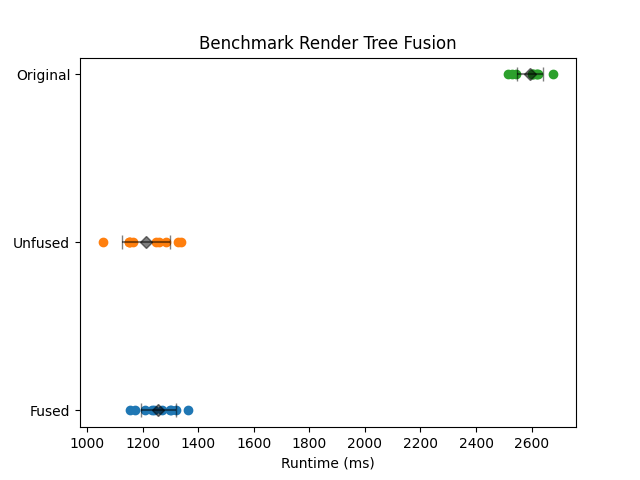
\includegraphics[height=8cm]{./img/rdt_fusion.png}
\caption{Comparison of original, rewritten but unfused, and fused runtimes for the render tree benchmark (n=1000 pages).}
\label{fig:bm-rdt}
\end{figure}

The code generated by the algorithm without applying fusion logically visits the same number of nodes as the input version, but fully accounts for the 51\% speedup. And although it is within the margin of error, it was even measured to be slightly faster than the fused version in this case, with mean runtime $\mu = 1212$ ms and $\sigma = 87$ ms. This means that enabling fusion could very well have no effect at all for this benchmark. This clearly affects the real-world benefit of applying this optimization.

Interestingly, the speedup also does not seem to be affected by the input size (other than the fact that there is a minimum size below which runtimes are too fast to be able to make meaningful measurements). This is not consistent with what would be expected for the traversal fusion optimization, nor is it consistent with the Grafter evaluation, in which larger inputs drastically increase speedup as expected \cite{SakkaSN019}. All of this indicates that the speedup is caused by something else. This is further discussed in \autoref{sec:bm-discussion}.

Although traversal optimization is thus unable to achieve real-world performance improvements for the render tree program, it can provide a measurable performance improvement in the best-case scenario benchmark. \autoref{fig:bm-full} shows that the fused version is significantly faster than both the input program and the version of the program that has gone through code synthesis with fusion disabled. On a binary tree of depth 17 ($2^{17} - 1$ nodes), the original program has a mean runtime of $\mu = 677$ ms with $\sigma = 51$ ms. Code synthesis without fusion achieves a speedup of approximately 16\% ($\mu = 571$ ms, $\sigma = 58$ ms), while fusion achieves a total speedup of 48\% ($\mu = 351$ ms, $\sigma = 44$ ms).\footnote{Two outliers $>1500$ ms have been removed for both the original and unfused versions. The fused version had no significant outliers.}

\begin{figure}
\centering
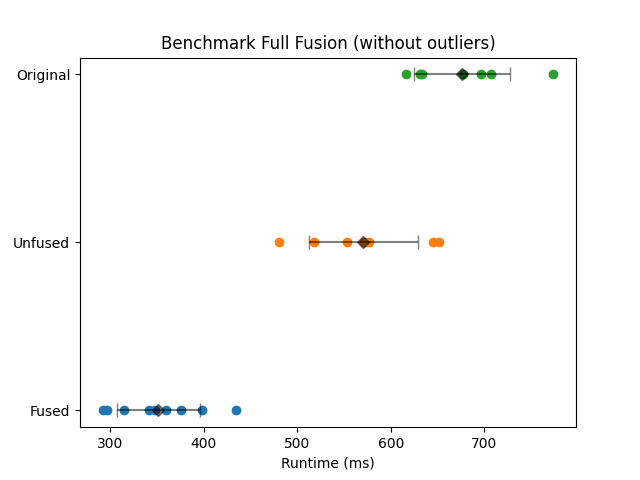
\includegraphics[height=8cm]{./img/full_fusion_no_outliers.png}
\caption{Comparison of original, rewritten but unfused, and fused runtimes for a synthetic benchmark that achieves full fusion (n=$2^{17} - 1$ nodes).}
\label{fig:bm-full}
\end{figure}

\section{Discussion}
\label{sec:bm-discussion}
Traversal optimization performs as expected in the best-case scenario benchmark. In the real-world render tree benchmark, we have seen that synthesizing code without enabling fusion can achieve a significant runtime speedup, while subsequently enabling fusion seems to have little to no further impact. These results require further investigation.

We also discuss the practical applicability of the traversal fusion optimization for strategic programming.

\subsection{Lack of Fusion Speedup}
The fact that traversal fusion significantly reduces the number of node visits in both the render tree and best-case benchmarks means that we also expected to see a significant speedup. The fact that this speedup is present in the best-case scenario benchmark, but not in the render tree benchmark, seems to indicate that traversal fusion introduces some other overhead.

It is not clear what the source of this overhead is, but it is most likely related to one of the following aspects in which the render tree benchmark differs from the best-case scenario benchmark. First, partial fusion requires more complex traversal functions with conditionals compared to unfused or fully fused programs. Simple traversal functions may be easier to optimize, have better interactions with the JVM, or simply perform better for any other reason. Second, the render tree benchmark contains many more node types, constructors, and rewrite rules. It is possible that this causes additional overhead, possibly in combination with any overhead already caused by partial fusion. We have not been able to identify the actual source of the overhead, and it is possible that there is another cause.

Another interesting theory is that there is another source of overhead unrelated to the traversals. For example, this could be the application of the rewrite rules themselves. Traversal fusion, as we have seen, cannot change the number of applications of rewrite rules. This source of overhead could be so large that the total traversal time is simply too small in comparison for traversal fusion to have a measurable effect. For example, suppose that there are 1000 traversal calls and 1000 rewrite rule applications, and traversal fusion reduces this to 500 traversal calls and 1000 rewrite rule applications. If the rewrite rules dominate the total runtime (e.g. they take $1$ ms each, while the traversal calls take $1$ ns each), we would expect no significant runtime impact due to traversal fusion.

To verify whether this is at least a plausible theory, we have created an alternate version of the render tree benchmark in which every traversal call includes a busy-wait of a certain amount of time. We then compare the version that has gone through code synthesis with fusion disabled with the fused version. The results of this comparison are shown in \autoref{fig:bm-add-time}. Indeed, artificially increasing the amount of time that the traversal calls take relative to the rest of the program increases the benefit of traversal optimization. Without additional traversal time, the versions have almost equal performance. At $5$ $\mu$s additional time, the fused version is 23\% faster, and at $20$ $\mu$s the fused version is approximately 31\% faster.

\begin{figure}
\centering
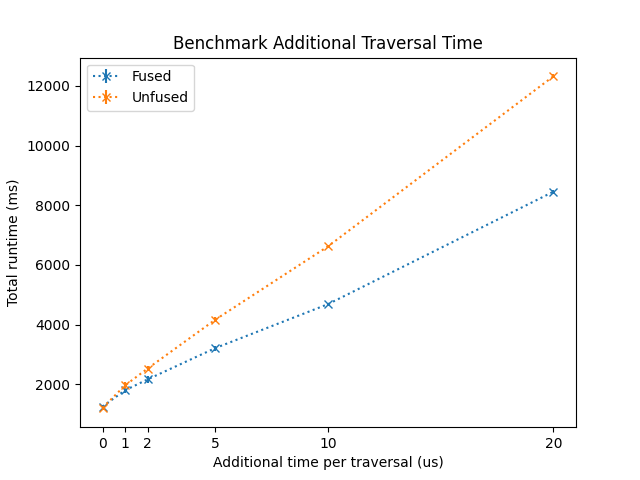
\includegraphics[height=8cm]{./img/add_traversal_time_full.png}
\caption{Comparison of unfused and fused mean runtimes for the render tree benchmark, with increasing additional traversal time (n=1000 pages).}
\label{fig:bm-add-time}
\end{figure}

\subsection{Code Synthesis Speedup}
Our theories to explain the lack of speedup due to traversal fusion do not explain the speedup that occurs after code synthesis without fusion. Although it is out of scope for this thesis to explore this speedup, it being unrelated to traversal fusion, it is certainly interesting. The most likely cause is an unexpected JVM interaction or some other Stratego-specific effect. Still, it may be interesting to investigate this speedup in the context of traversal fusion in the future, as we cannot rule out that it is related to the lack of speedup we have seen for traversal fusion.

\subsection{Further Discussion}
Although we can conclude that traversal optimization is possible in strategic programming, the results of this evaluation raise concerns about practical applicability.

For compiler designers, implementing additional optimizations means investing time, an increase in compiler complexity, and an increase in compiler overhead. As such, implementing an optimization is always a trade-off, and this only makes sense if the optimization provides a significant benefit relative to the cost of implementing it.

The lack of speedup in the render tree benchmark indicates that there is little point in performing fusion for such a program in a real-world scenario. The traversal fusion optimization itself is also relatively complex, and its performance scales poorly with input program size (because it finds all possible fusions). The complexity of the optimization is certainly an important factor: it increases the chances of compiler bugs, which could lead to potentially incorrectly compiled code. Compiler bugs are notoriously hard to deal with for programmers and could carry significant consequences if not caught. If there is indeed little benefit to performing the optimization, it would be hard to conclude that the trade-off favors implementing the traversal fusion optimization in this case.

On the other hand, we have identified two cases in which fusion does provide a significant speedup (namely, when performing full fusion on a simpler program, and when artificially increasing traversal time). These benchmarks are further removed from real-world applications, but in theory these situations certainly could occur. In addition, we have not identified situations in which fusion creates a slower program. For a programmer writing programs in a strategic language, there is little cost in performing the optimization (other than increased compiler runtime), meaning even a relatively small chance of increased performance could certainly be worth it.

In any case, we would argue that it is at least possible in theory that the issue of fusion not providing a speedup could be solved. If it can, this would certainly shift the trade-off to be in favor of implementing it, because the performance increase can be very significant. If this issue cannot be solved, it could be worth at least investigating whether there exists a test that can be performed quickly to predict whether fusion could provide a benefit for a certain program.

We feel that it is fair to conclude that, although there are valid concerns about the practical applicability that would prevent this optimization from being implemented right now, it is too early to give up on it entirely in strategic programming.

\section{Validity}
There are two main factors that can impact the validity of this evaluation.

First, a significant factor is the generalizability of these results. We aim to assess the effect of the traversal fusion optimization on strategic programs in general. To do this, we evaluate an implementation on a subset of one strategic programming language, Stratego. On top of that, the render tree benchmark is based on a domain in which strategic programming languages are normally used, but may not be fully representative (and it has also been selected to fit within the supported subset of Stratego). We do note, in defense of this approach, that:
\begin{itemize}
    \item It is true that the performance impact may differ depending on many factors, but the core result of whether traversal fusion works at all is easily generalizable to all strategic languages. We have shown that for a large program, similar to real-world applications, the algorithm can correctly identify fusion opportunities and synthesize fused traversal code.
    \item Although the render tree benchmark has been carefully selected to be representative, the performance of the traversal fusion optimization may still differ significantly between programs. This depends mainly on the number of fusion opportunities available for that program. That does mean that the optimization may be more effective for certain types of programs than it is for others. However, this is true for for most optimizations. Although of course a simplification, we could say that traversal fusion suffers from a lack of fusion opportunities in the same way that an optimization such as loop unrolling suffers from a lack of loops to unroll. In general, the optimization may still be viable.
\end{itemize}

Second, the goal of measuring the impact of the traversal fusion optimization can be adequately achieved by measuring the program runtime. However, this is the overall program runtime, which is subject to significant variance. We have noticed that Stratego programs always seem to have a significant variance in runtime. On top of that, the overall program runtime includes operations such as reading the input data. Although these operations are identical for each benchmark that is compared, they may introduce additional variance in the data. On the other hand, variance in the program runtime is also controlled by including warm-up runs through JMH. Still, variance remains a significant factor, and four significant outliers had to be excluded from the best-case scenario benchmark.
% !TEX root = document.tex

\chapter{\label{chap:related-work}Related work}
\label{chap:rw}
In this section, work related to tree traversal fusion is discussed. These are works that discuss fusions of any kind applied to trees (not necessarily in a strategic or functional context), and some works that discuss fusion in general.

\section{Fusion in general}
Here, we discuss some more distantly related work on fusion, showing different approaches.

\subsection{Fusion in a strategic language}
It is possible to fuse the innermost strategy (traversal) with its rules in Stratego \autocite{JohannV01}. This fusion reduces the number of times the innermost strategy has to revisit nodes by keeping track of which parts are already in a normal form (which will not change anymore). This implies that it is at least possible and feasible to optimize some traversals under some conditions in Stratego. Note, however, that this fusion is not \textit{exactly} a fusion as defined in this thesis: it does not say anything about combinations of multiple, possibly different, strategies. Instead, it only looks at a single traversal and optimizes that one traversal.

\subsection{Deforestation and Circular Programming in Functional Programming}
Research has been done on combining deforestation and circular programming to achieve fusion in functional programming.

\paragraph{Deforestation}
Many functional programs rely on the creation of intermediate data structures because functional languages do not (in general) allow for mutation. The term deforestation, then, describes the elimination of these intermediate data structures such as trees during a computation \autocite{FernandesCSP15}.

\paragraph{Circular programming}
Circular programming is the technique of using circular definitions in a lazy language and allowing the language to compute a correct and terminating evaluation order (if it exists). It has been shown that ``any algorithm that performs multiple traversals over the same data structure can be expressed in a lazy language as a single traversal circular function" \autocite{FernandesPS07}. Note that this does not necessarily imply that the number of actual performed traversals is reduced (although it can be), depending on the selected evaluation order. The only guarantee is that at least the algorithm can be \textit{expressed} as a single circular traversal.

\paragraph{Combining deforestation and circular programming}
Functions that generate intermediate data structures can and do, of course, also traverse these data structures. This means that, while the intermediate data structure may be optimized out after deforestation, the actual computing traversal does not necessarily disappear. Some research has been done on combining deforestation with circular programming to both eliminate intermediate data structures and simultaneously reduce the number of traversals needed to compute the final result \autocite{FernandesPS07}.

As an example, consider the problem of replacing every node in a tree of integers with the minimum value in the tree. It is possible to replace every node with the minimum value in a single traversal by computing the minimum value lazily. Or, in other words, the nodes are all updated while traversing the tree to find the minimum, but their concrete value is only computed once the entire tree has been traversed and, as such, the minimum value has been found.

Although this method of deforestation with circular programming is effective in fusing traversals, it is quite different from what has been presented in this paper. The circular programming method does not look at what the specific traversal is (top-down, bottom-up, etc.) and then reason about that traversal generically. Instead, it changes the actual functions (or what would be rewrite rules in the case of strategic programming) to use lazy computation, and in the process reduces the number of required traversals. As such, it does not provide information about the nature of these traversals themselves or how they interact with each other.

Still, it may be worth investigating whether this method can work in strategic programming.

\subsection{Other Fusion in Functional Programming}
Several other fusion optimizations have been developed in functional programming. Although not directly relevant to (generic) tree traversal fusion, they are still conceptually related by virtue of performing \textit{a} fusion.

\textbf{Generalized Deforestation} There is a generalization of deforestation to all first-order and higher-order functional programs. This model views all parts of a program as safe or unsafe producers or consumers, identifying fusion opportunities for subterms of any expression\cite{Chin92}. Although this generalization may not be directly relevant for the problem presented in this thesis, the concept of automatically classifying subterms as safe or unsafe may be worth investigating.

\textbf{Stream fusion} Stream fusion was ``the first truly general solution" to fusion for algorithms over sequences (such as lists) in functional programming\cite{Mainland17}. Its main principle is ``transforming recursive structures into non-recursive co-structures" (i.e. streams) that can be more easily fused\cite{Mainland17}. This method has since been expanded upon in the form of generalized stream fusion, which computes a bundle of multiple different streams. This allows a choice for the most efficient representation and opens up the possibility for parallelization through Single Instruction, Multiple Data (SIMD) instructions. 

We have seen that tree traversal fusion is fundamentally different from fusion for sequences such as lists, but it may still be possible to adapt these concepts to traversal fusion. For example, could analyzing a tree as its co-recursive counterpart make fusion easier? At the very least, even if these concepts cannot be directly adapted, exploring the use of SIMD instructions for tree traversal fusion could be very interesting.

\section{Tree Fusion}
Research on tree fusion that is more closely related to the topic of this thesis has also been done, although not in the context of strategic programming. We will discuss some of it here.

\subsection{TreeFuser and Grafter}
The research done on TreeFuser and Grafter has been used extensively throughout this thesis. They provide a framework for automatic traversal fusion in a C++-like imperative language, using a dependency analysis approach \cite{SakkaS017, SakkaSN019}. Refer to \autoref{sec:towards-a-solution} for a more thorough explanation.

\subsection{Other ways}
A few other approaches to tree fusion have also been developed.

RETREET \cite{WangLZQ21} constructs a monadic second-order logic over trees, and uses a solver to identify fusion opportunities. The authors note that the main benefit of RETREET is that it is a more general framework with fewer limitations compared to approaches such as TreeFuser. The algorithm heuristically enumerates possible fusions, and the solver checks these for correctness. They evaluate RETREET on real-world benchmarks such as CSS minification, but only verify that the identified optimizations are correct. This approach is certainly promising, and it may also be possible to apply it to strategic programming. Of course, it would be worth verifying whether this approach can really find more fusion opportunities in the context of strategic programming, or at least facilitates the implementation of additional syntactic features.

HECATE \cite{ChenLFB22} is a solver-aided Domain Specific Language (DSL). Traversals written in this DSL are translated to a counterexample-guided solver that identifies fusion opportunities. The authors compare it directly to Grafter. While they identify the same fusion opportunities, meaning the performance of the fused code is largely identical, they note that their fusion algorithm is significantly faster (on average 8.0x faster than Grafter). HECATE also provides additional interesting options, such as support for parallelization. Enabling parallelization for the render tree benchmark (used for the Grafter evaluation, as well as in this thesis) increases performance by an additional 23\%.
% !TEX root = document.tex
\chapter{\label{chap:conclusion}Conclusion}

This thesis presents an algorithm for traversal fusion in strategic programming languages, answering the research question: `Can generic traversal fusion be performed in strategic programming languages, and what is the impact of this optimization on strategic programs?'

To answer the research question, an algorithm that can perform traversal fusion in a strategic programming language was developed based on previous work (TreeFuser and Grafter \cite{SakkaS017, SakkaSN019}). The method relies fundamentally on a dependency analysis of the input program. This dependency analysis can identify opportunities to fuse traversals without altering program results. A proof-of-concept implementation of this algorithm for the Stratego language was implemented and evaluated on several synthetic benchmarks.

We find that traversal fusion can indeed be performed in strategic programming languages but that performance impact in real-world use cases is absent. In some cases, such as when performing full fusion, or when the portion of total runtime taken up by the traversal calls is relatively large, traversal fusion can provide a measurable mean runtime decrease ($>50\%$). However, these situations are unlikely to occur in real programs. In a render tree benchmark simulating a real-world use case, node visits were reduced by over 40\%, but no speedup was measured\footnote{At least, no additional speedup in addition to the unexplained speedup due to code synthesis}.

Compared to traversal fusion for imperative languages, in which traversal fusion provides a significant performance benefit, these results are surprising. The most likely theories to explain the lack of speedup are that fusion introduces some unexpected overhead in Stratego, or that other parts of the program (unrelated to the traversal) take an unexpectedly large amount of time. In either case, we do believe that it is worth investigating these results in more detail, and that it is too early to conclude that the traversal fusion optimization is entirely unviable in strategic programming.

Still, we have shown that traversal fusion can at least be performed on generic traversals in strategic programming languages, laying the foundation for future research in this area.

\section{Future Work}
We make the following suggestions for future work.

First, we recommend that the unexpected lack of performance be further investigated. There are a few different possibilities:
\begin{itemize}
    \item Perform a more thorough investigation into Stratego, the specific code generated by this algorithm, and analyze it in more detail using a profiler
    \item Create more synthetic benchmarks to analyze the performance of different programs, to create a better understanding of which aspects create performance issues
    \item Implement this algorithm in a different strategic programming language to assess whether the unexpected results are specific to Stratego
\end{itemize}

Should it turn out that the performance issues can be resolved and that traversal fusion is indeed a viable optimization for strategic programming, there are several aspects of the algorithm itself that can also be improved. These are, in no particular order:
\begin{itemize}
    \item If the optimization is viable, it would be a good idea to implement a version of the algorithm in the Stratego compiler, that also operates on the full language (not a subset). This would require adding support for additional syntax features.
    \item Currently, rewrite rules are analyzed as a single large statement that cannot be split. Automatically splitting rewrite rules into multiple statements, possibly based on a heuristic, may increase the number of opportunities for fusion.
    \item It may be a good idea to implement optimizations for the algorithm itself. The POC was not developed with performance in mind, and if it is to run as part of the compiler, it would benefit from increased performance.
    \item Assess whether there are better code generation strategies. It is possible that the current matching approach to congruence does not create the fastest possible code. 
    \item Assess whether certain topological orders are better than others. The code generation currently picks a random topological order after fusion. It may turn out that certain traversal orders are simply better.
    \item Attempt to develop heuristics to determine which fusion opportunities are best. The algorithm currently creates every possible fusion, and then picks the fusion with the most amount of fused nodes. This is not a great strategy, as it scales poorly. A good heuristic to pick certain fusion opportunities over others is important to make this optimization practically useful.
    \item Attempt to use results from this algorithm to find new fusion rules that \textit{always} work. We are not certain of how likely this is, but it could be the case that there are certain fusions that are always legal that can be identified using this algorithm. It would at least be interesting to explore this.
\end{itemize}

\printbibliography{}


\hidefromtoc
\chapter*{\label{chap:acronyms}Acronyms}
\addcontentsline{toc}{chapter}{Acronyms}

% Syntax:
% \acro{<acronym>}[<short form>]{<long form>}
% \acroplural{<acronym>}[<short plural>]{<long plural>}
\begin{acronym}

    % Order manually:

    % Acronyms here
    \acro{AI}{Artificial Intelligence}
    \acro{AST}{Abstract Syntax Tree}
    \acro{ATerm}{Annotated Term}
    \acro{DSL}{Domain Specific Language}
    \acro{EEMCS}{Electrical Engineering, Mathematics \& Computer Science}
    \acro{JMH}{Java Microbenchmark Harness}
    \acro{JVM}{Java Virtual Machine}
    \acro{POC}{Proof-Of-Concept}
    \acro{SIMD}{Single Instruction, Multiple Data}
    

\end{acronym}
\unhidefromtoc

% Usage:
% \ac{<acronym>} - Singular acronym, expanded on first use, e.g. "API".
% \acp{<acronym>} - Plural acronym, e.g. "APIs"
% \acf{<acronym>} - Expanded form, e.g. "application programming interface (API)".
% \acfp{<acronym>} - Expanded form plural.
% \acs{<acronym>} - Short form, e.g. "API"
% \acsp{<acronym>} - Short form plural.
% \acl{<acronym>} - Long form, e.g. "application programming interface"
% \aclp{<acronym>} - Long form plural.
% \acsu{<acronym>} - Short form, and marks it as used
% \aclu{<acronym>} - Long form, and marks it as used

% \acresetall{} - Reset all acronyms to use their expanded form on next use.
% \acused{<acronym>} - Set the acronym as used, to use their short form on next use.

%\appendix
%\def\chaptername{Appendix}
%\include{A00-appendix}

\end{document}
